\documentclass{article}
\usepackage{ctex}  % 支持中文
\usepackage[a4paper,margin=2cm]{geometry}
\usepackage{xcolor}
\usepackage{listings}
\usepackage{caption}
\usepackage{graphicx}
\usepackage{float}
\usepackage{rotating}
\usepackage[inkscapelatex=false]{svg}

% 定义代码块注解格式
\renewcommand{\lstlistingname}{代码}

% 定义颜色
\definecolor{codegreen}{rgb}{0,0.6,0}
\definecolor{codegray}{rgb}{0.5,0.5,0.5}
\definecolor{codepurple}{rgb}{0.58,0,0.82}
\definecolor{backcolour}{rgb}{0.95,0.95,0.92}

% 定义 listings 风格，可以定义多个
\lstdefinestyle{mystyle}{
	% backgroundcolor=\color{backcolour},           % 代码块的背景色（此行被注释掉）
	commentstyle=\color{green!60!black},            % 注释文字的颜色（混合色：50%红+50%绿+50%蓝）
	keywordstyle= \color{blue!70},                  % 关键字（如 def, if, return 等）的颜色（70% 蓝色）
	numberstyle=\tiny\color{codegray},              % 左侧行号的字体大小和颜色（tiny 字号，灰色）
	stringstyle=\color{codepurple},                 % 字符串（如 "Hello"）的颜色（紫色）
	basicstyle=\ttfamily\footnotesize,              % 代码的基础字体：等宽字体 + 脚注大小
	breakatwhitespace=false,                        % 是否只在空白处换行（false = 可以在任意字符处换行）
	breaklines=true,                                % 对过长的代码自动换行（true = 开启自动换行）
	captionpos=b,                                   % 标题位置：b = bottom（底部），也可设为 t（顶部）
	keepspaces=true,                                % 保留代码中的空格（不压缩多个连续空格）
	numbers=left,                                   % 在左侧显示行号（也可设为 right 或 none）
	numbersep=5pt,                                  % 行号与代码之间的距离（5 个点）
	showspaces=false,                               % 是否显示空格符号（false = 不显示）
	showstringspaces=false,                         % 是否在字符串内显示空格符号（false = 不显示）
	showtabs=false,                                 % 是否显示制表符（tab）符号（false = 不显示）
	tabsize=2,                                      % 制表符（tab）对应的空格数（1 个 tab = 2 个空格）
	frame=single                                    % 代码块边框样式：single（单线框），也可用 none（无框）或 shadowbox（阴影框）
}

\lstset{style=mystyle}

\begin{document}
	\begin{center}
		{\LARGE 高铁订票管理系统开发文档}
	\end{center}
	
	\vspace{1cm}
	
	\begin{tabular}{rl}
		课程名称： & 程序设计综合实践 \\
		项目名称： & 高铁订票管理系统 \\
		班级： & 信息工程学院计算机科学与技术一班 \\
		团队成员：& 王宇豪（1231001024）、熊江伟（1231001026）\\
		编程语言：& QML、Javascript、C++ \\
		开发周期： & 2025.8-2025.12
	\end{tabular}
	\\
	\\
	\\
	\tableofcontents
	\newpage
	
	\section{项目概述}
	本项目是一个基于Qt6（C++）和QML开发的高铁订票管理系统。项目采用了经典的\textbf{前后端分离架构思想}，前端使用Qt框架下提供的主流前端标记型语言QML进行前端逻辑的开发，后端使用C++处理核心业务流程、数据存取和算法实现。系统支持普通用户（订票、查询、订单管理、乘车人管理）和管理员（车次管理、订单管理、用户管理）两种角色的操作。项目开发使用Git工具进行版本控制，使用GitHub远程仓库进行代码备份。
	
	\textcolor{red}{\textbf{源码已打包成EXE可执行文件。可以直接在\texttt{src/build/Desktop\_Qt\_6\_9\_3\_MinGW\_64\_bit-Release}目录下双击\texttt{appRailwaySystem.exe}执行！}}
	
	\section{需求分析}
	\subsection{功能性需求}
	\subsubsection{普通用户功能}
	\begin{figure}[H]
		\centering
		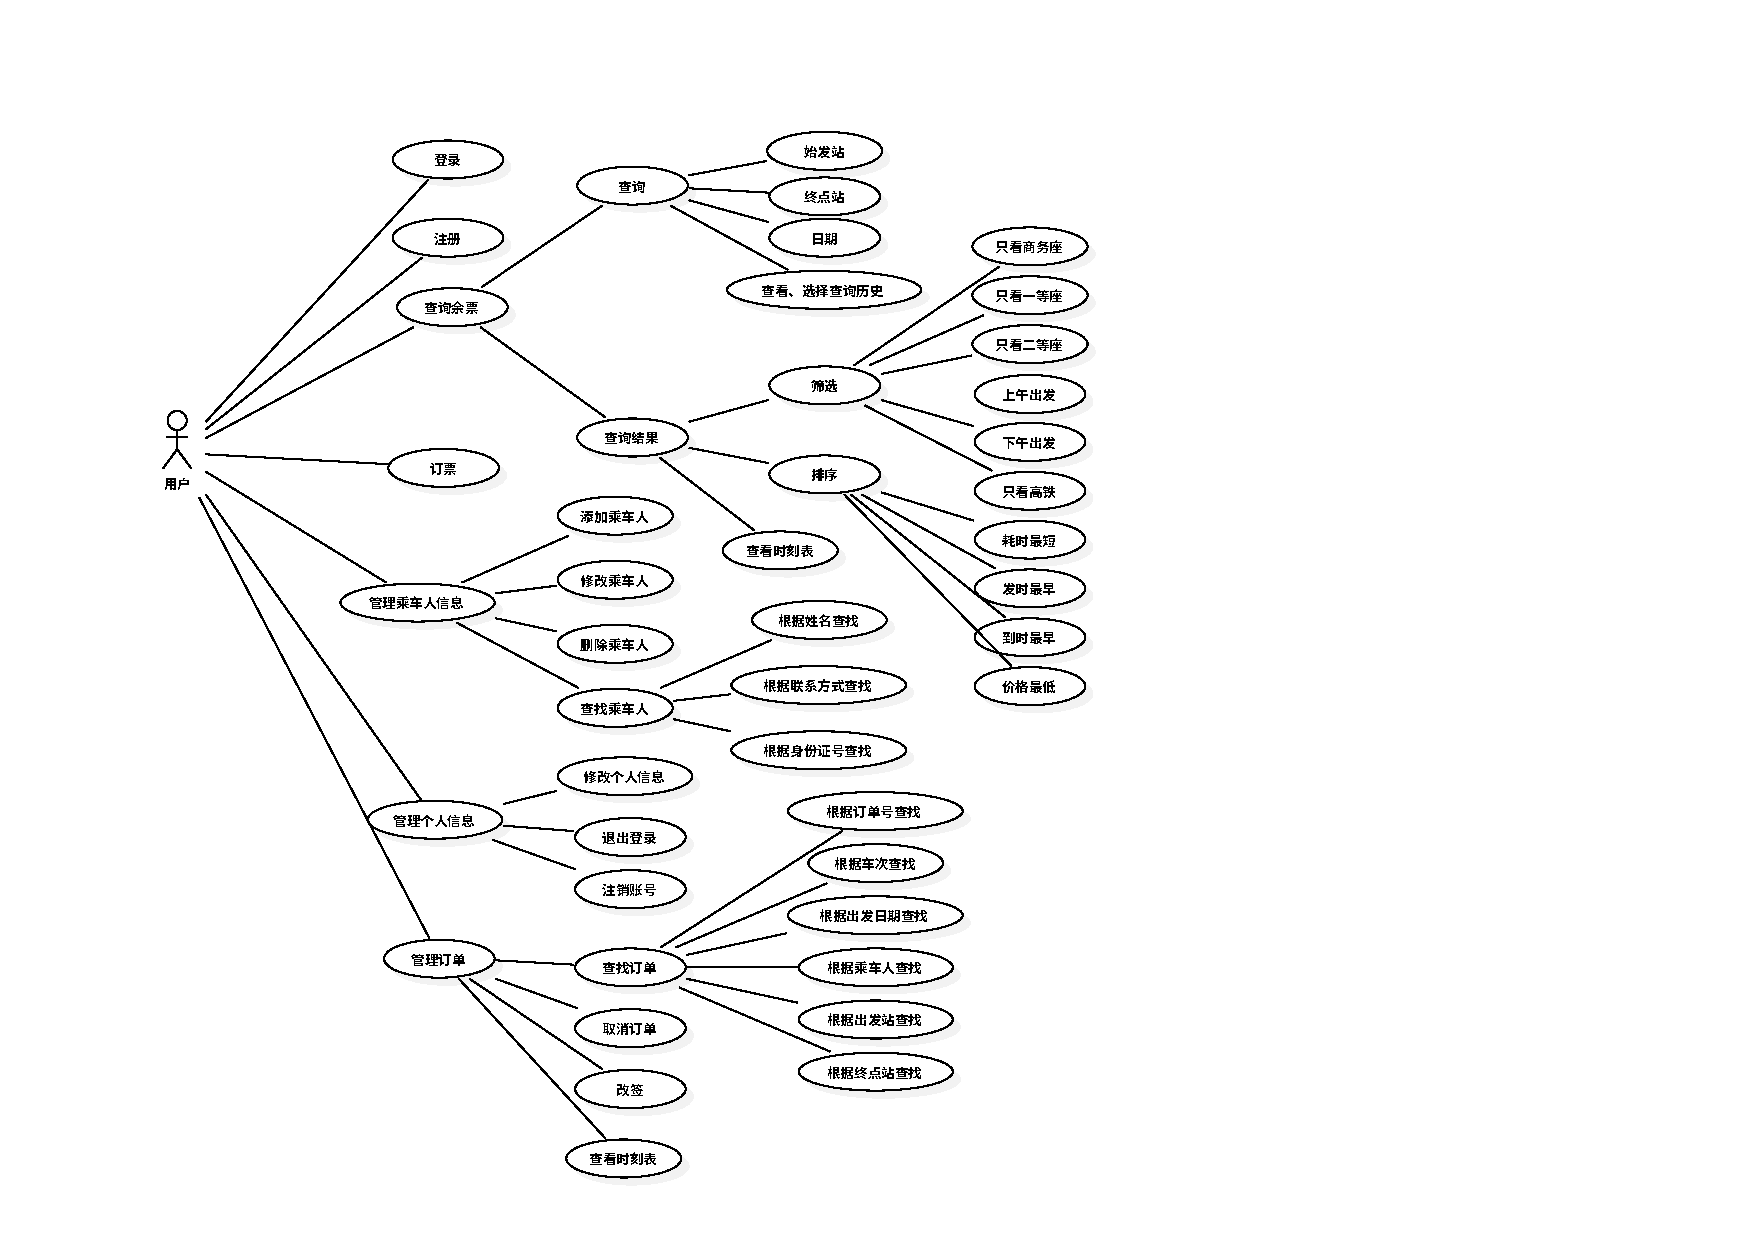
\includegraphics[width=1.5\textwidth]{用户用例图.pdf}
		\caption{用户用例图}
	\end{figure}
	
	普通用户作为系统的核心使用者，主要完成车票查询与出行相关的全流程操作。用户可进行账号注册与登录，在输入始发站、终点站与出行日期等条件后查询余票，并对查询结果进行筛选与排序、查看时刻表及使用查询历史记录以提升检索效率。在此基础上，用户可完成订票操作。
	
	此外，系统为普通用户提供信息管理能力：用户可维护乘车人信息（如新增、修改、删除与查找），并可对个人信息进行管理（如修改资料、退出登录与注销账号）。在订单环节，用户可对订单进行查询与管理，包括查看订单与相关时刻信息、取消订单以及改签等操作，从而形成“查询—订票—管理”的闭环使用体验。以下是一些主要功能的详细介绍（\textbf{界面图片与前期设想和手工绘制一致}。
	
	\begin{figure}[H]
		\centering
		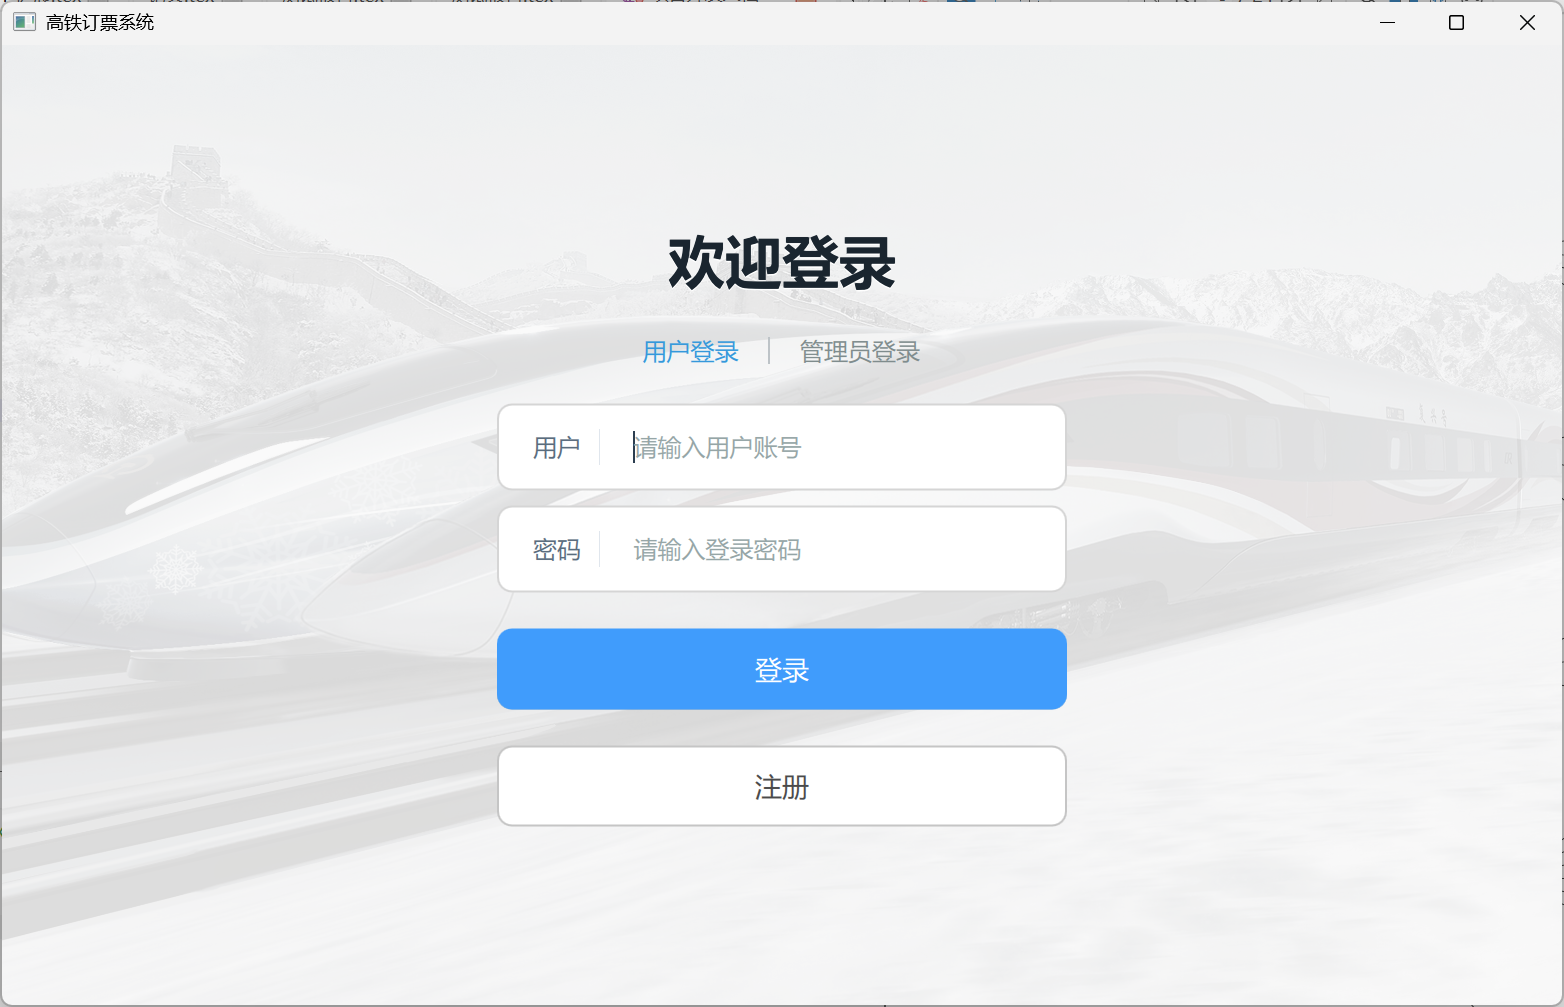
\includegraphics[width=0.7\textwidth]{用户登录功能.png}
		\caption{用户登录功能}
		\label{用户登录功能}
	\end{figure}
	
	\paragraph{登录} 如图\ref{用户登录功能}所示，用户在登录界面点击“用户登录”，通过在输入框中输入用户名和密码，点击登录后能够进行登录操作。如果用户名和密码正确，则登录成功，进入首页；否则系统会以弹窗提示的形式告诉用户出现的问题，由用户进行修改。
	
	\begin{figure}[H]
		\centering
		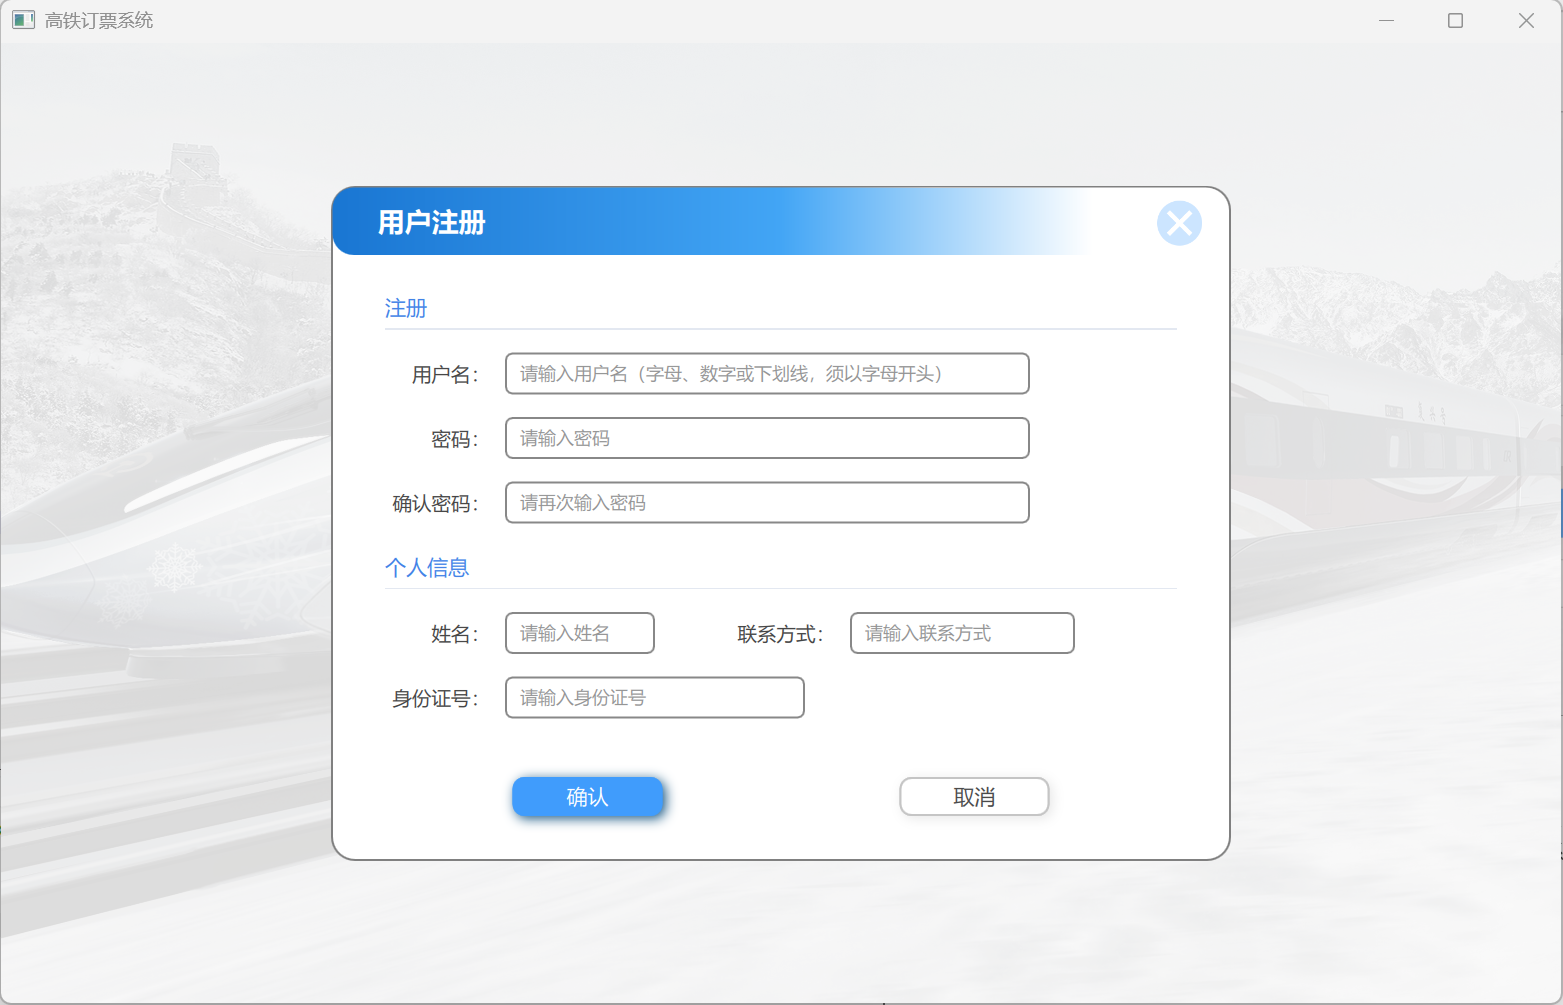
\includegraphics[width=0.7\textwidth]{用户注册功能.png}
		\caption{用户注册功能}
		\label{用户注册功能}
	\end{figure}
	
	\paragraph{注册} 用户如果没有账号，可点击登录界面下方的注册按钮，弹出注册窗口，如图\ref{用户注册功能}所示。用户需要在其中输入用户名、密码、个人信息，点击确认后即可注册自己的账号。
	
	\begin{figure}[H]
		\centering
		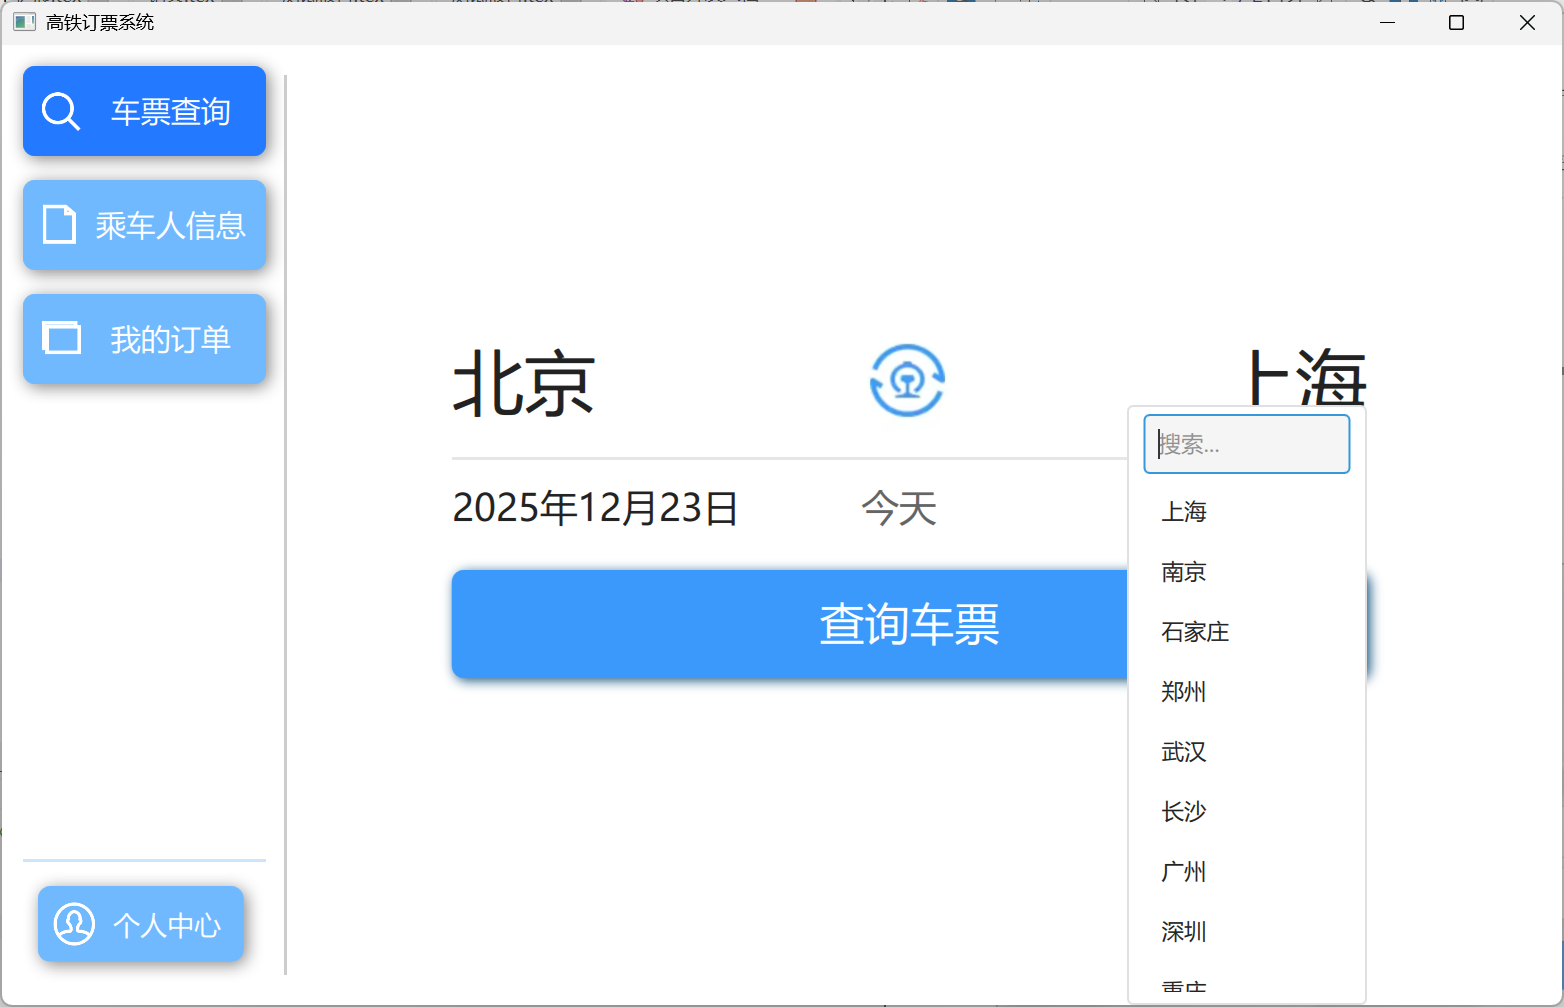
\includegraphics[width=0.7\textwidth]{查询余票功能.png}
		\caption{查询余票功能}
		\label{查询余票功能}
	\end{figure}
	
	\begin{figure}[H]
		\centering
		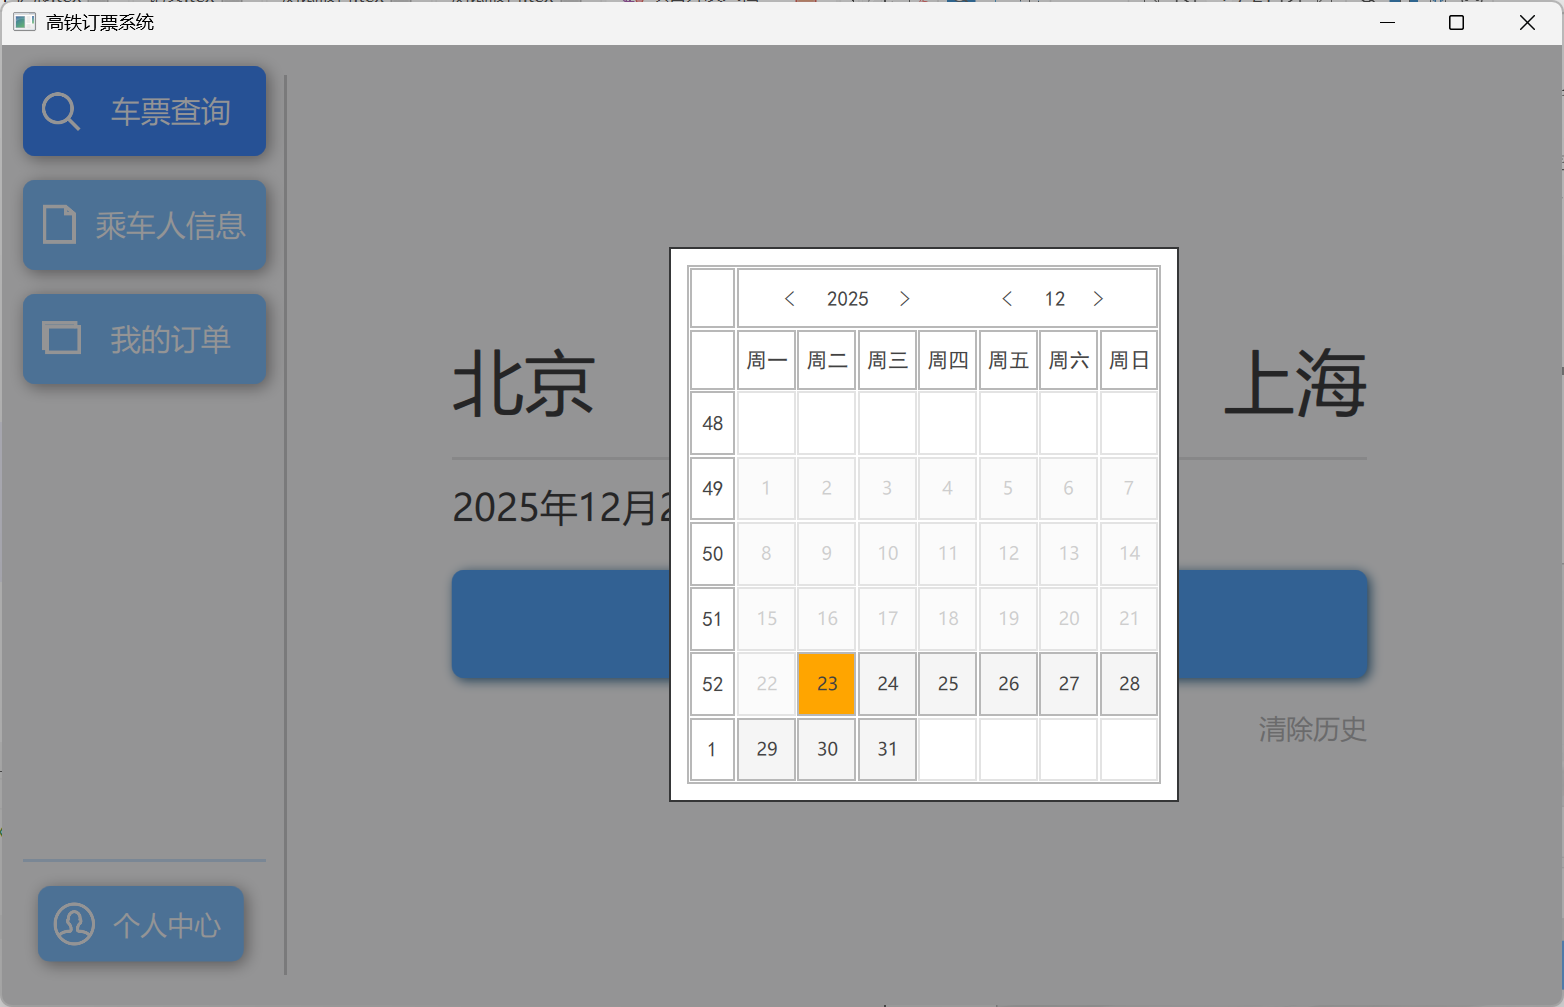
\includegraphics[width=0.7\textwidth]{选择查询日期.png}
		\caption{选择查询日期}
		\label{选择查询日期}
	\end{figure}
	
	\paragraph{查询余票} 用户登录后自动跳转到查询余票界面，如图\ref{查询余票功能}所示。在该界面，用户点击城市名即可弹出下拉列表，在列表中点击对应的城市即可更新城市名，并且考虑到城市数量过多导致列表过长，还给用户提供了列表搜索功能，搜索对应的城市即可模糊匹配出城市子集，再由用户选择。点击中间的logo可以交换出发城市和终点城市。另外，查询余票界面还提供查询历史功能，用户每进行一次查询操作，都会保存该查询历史，单次可保存最多3个查询历史，点击查询历史，即可直接将历史应用到当前查询的起末城市。用户点击右方的清除历史，即可清除所有查询历史。除了选择起末城市，用户点击下方日期即可弹出日历，如图\ref{选择查询日期}所示。用户在日历中可以确定要查询的日期。日期右边会提示日期为今天、明天或后天，或星期几（若距离今天超过3天）。
	
	\begin{figure}[H]
		\centering
		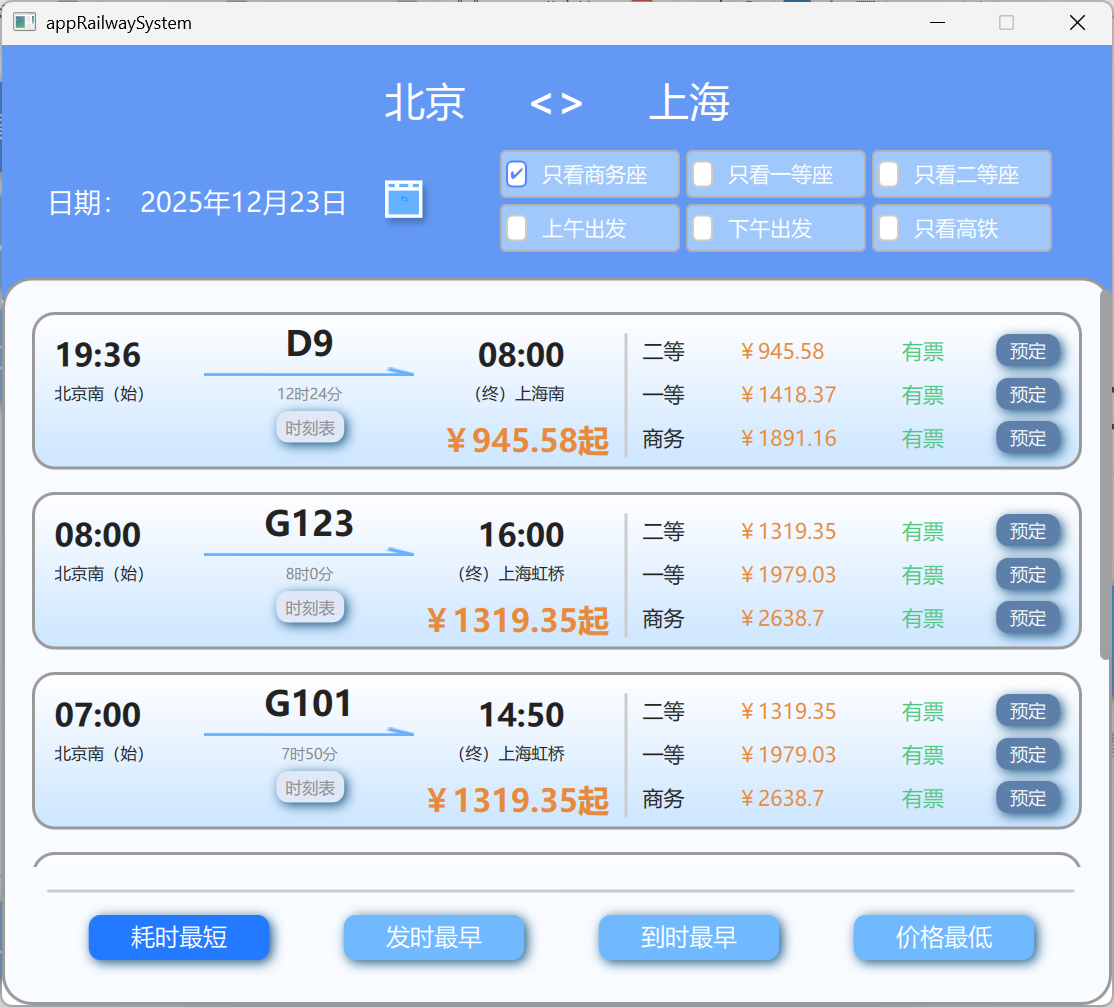
\includegraphics[width=0.7\textwidth]{查看余票查询结果.png}
		\caption{查看余票查询结果}
		\label{查看余票查询结果}
	\end{figure}
	
	\paragraph{查看余票查询结果} 用户点击查询后，根据选择的城市、日期查询余票，在新的窗口中弹出余票查询结果，如图\ref{查看余票查询结果}所示。用户点击最上方的\texttt{<>}按钮即可交换起末城市并重新获取查询结果。点击左上角的日历符号，同样能弹出日历窗口重新选择查询日期。右上角的筛选按钮点击后即可应用对应筛选，筛选出符合要求的余票。最下方的排序按钮点击后可以按照对应规则对余票进行排序。用户可以再次界面自由浏览余票信息、查看时刻表和点击预订。
	
	\begin{figure}[H]
		\centering
		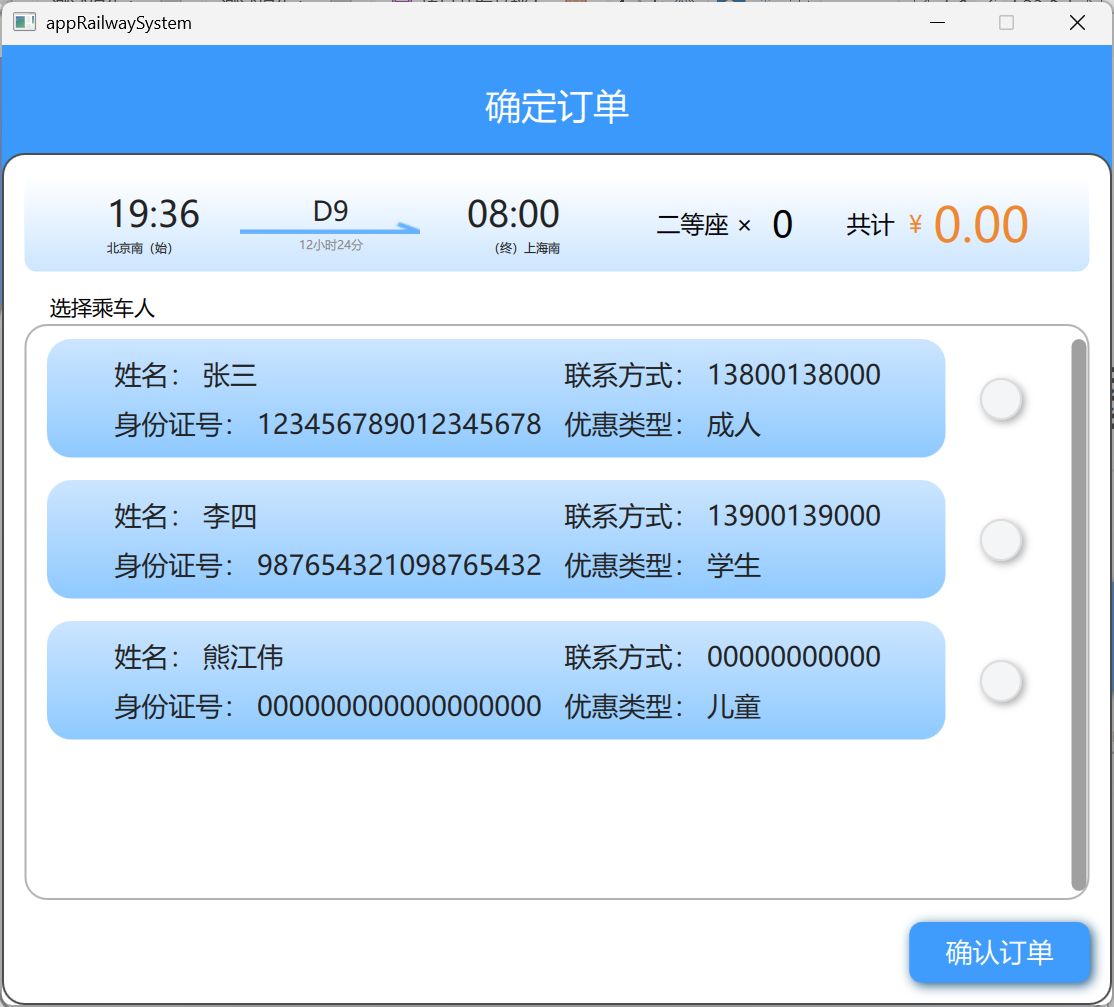
\includegraphics[width=0.7\textwidth]{选择乘车人功能.png}
		\caption{选择乘车人功能}
		\label{选择乘车人功能}
	\end{figure}
	
	\begin{figure}[H]
		\centering
		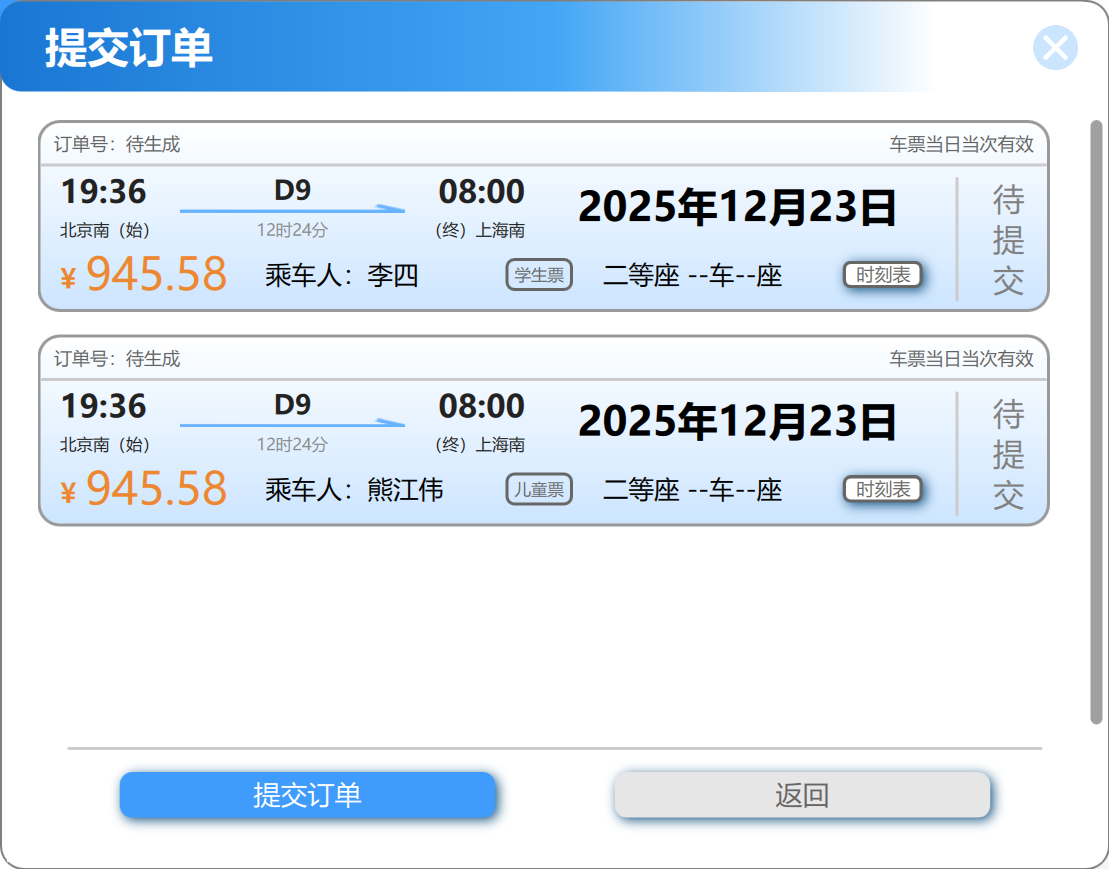
\includegraphics[width=0.7\textwidth]{提交订单功能.png}
		\caption{提交订单功能}
		\label{提交订单功能}
	\end{figure}
	
	\paragraph{选择乘车人功能} 用户在余票查询结果页面点击对应余票的“预订按钮”后，系统会弹出“确定订单”窗口，如图\ref{选择乘车人功能}所示。用户在该界面可以选择若干乘车人（仅可选择当前时间段处于空闲的乘车人，即无待乘坐订单）乘坐。点击确定订单后，系统弹出“提交订单”窗口，如图\ref{提交订单功能}所示，给用户展示待提交订单，用户再次点击确认后，系统开始分配座位号、分配订单号并创建订单，完成订票。
	
	
	\begin{figure}[H]
		\centering
		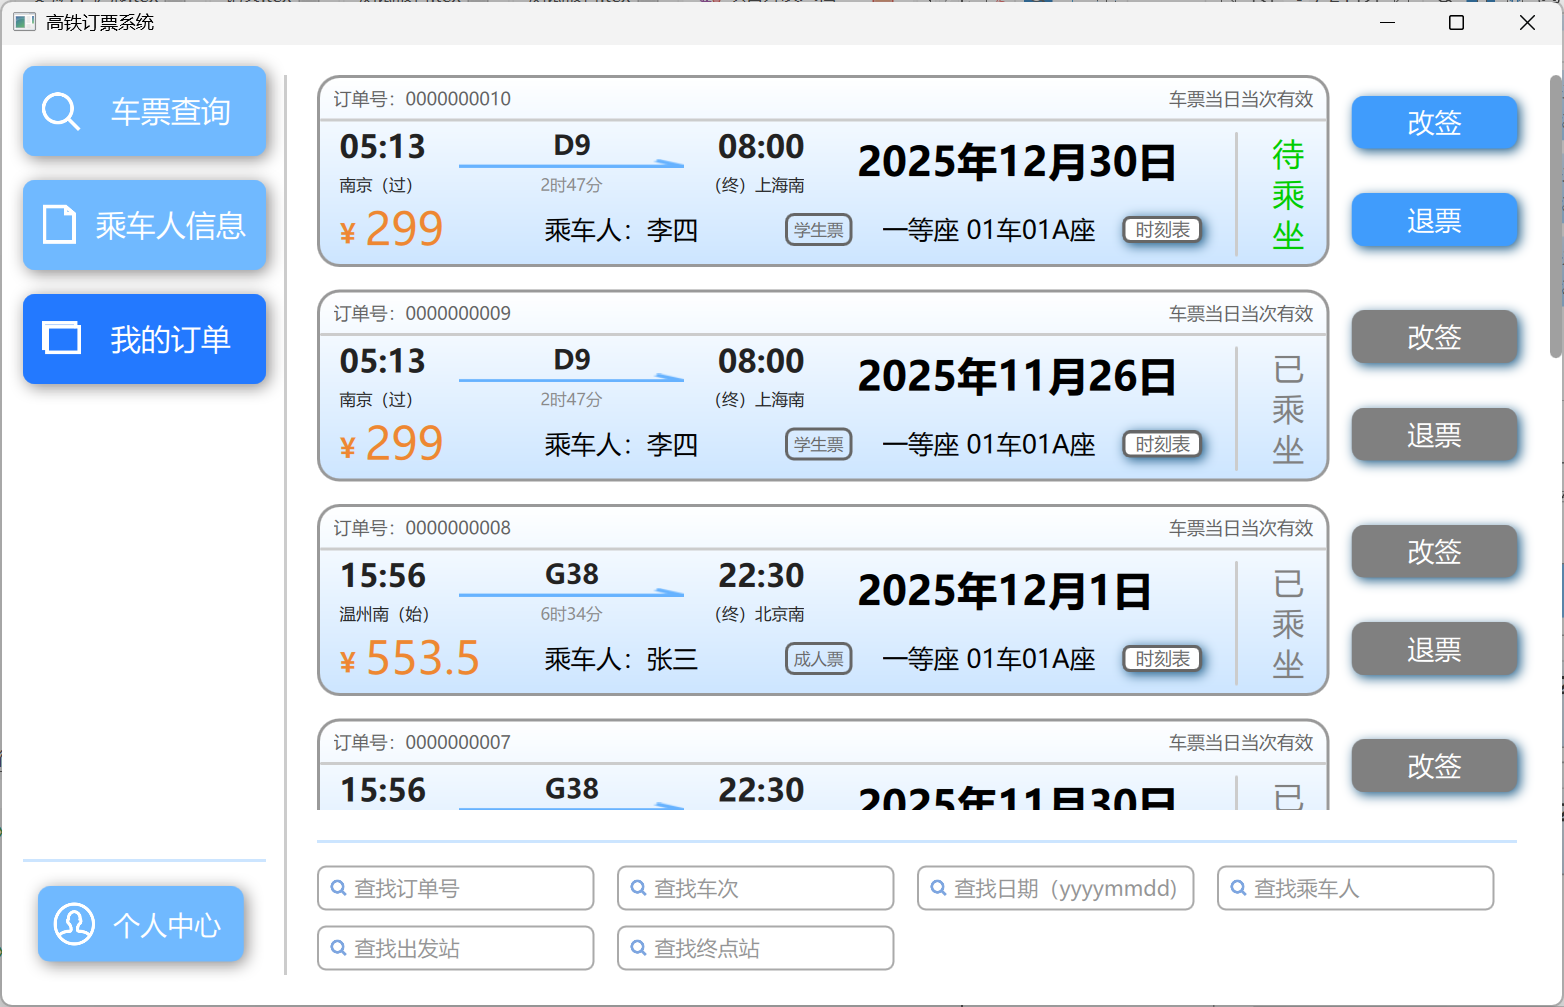
\includegraphics[width=0.7\textwidth]{我的订单管理功能.png}
		\caption{我的订单管理功能}
		\label{我的订单管理功能}
	\end{figure}
	
	\paragraph{我的订单管理功能} 用户点击侧边栏切换当前页面为“我的订单”，即可查看用户下的所有订单，如图\ref{我的订单管理功能}所示。用户在该界面可以查看订单信息，在最下方的搜索框中可以根据某些字段对订单进行搜索和筛选（支持多条件搜索）。每个订单都有改签和退票功能。点击退票后即可取消该订单，\textbf{点击改签后，会根据当前订单的起末站和出发日期，直接调用查询余票功能，弹出余票查询结果页面，由用户完成整个订票逻辑，即可实现改签}。
	
	\begin{figure}[H]
		\centering
		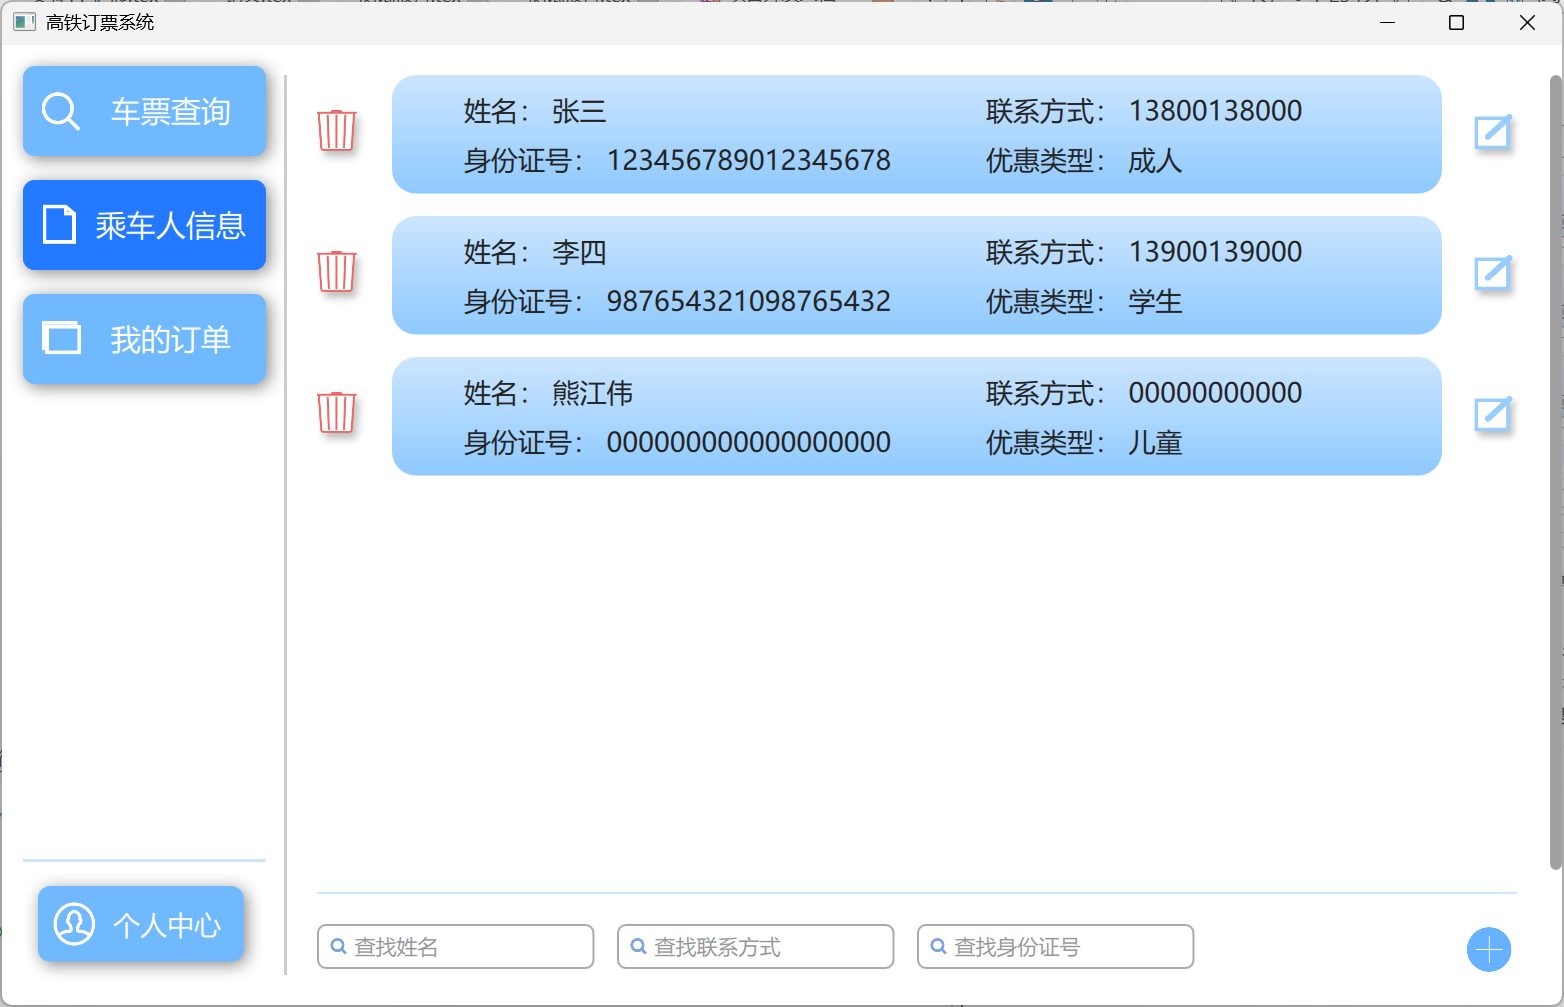
\includegraphics[width=0.7\textwidth]{乘车人信息管理功能.png}
		\caption{乘车人信息管理功能}
		\label{乘车人信息管理功能}
	\end{figure}
	
	\paragraph{乘车人信息管理功能} 用户在侧边栏切换当前页面为“乘车人信息”，即可查看用户下的所有乘车人信息，如图\ref{乘车人信息管理功能}所示。用户在该节目可以查看乘车人信息，在最下方的搜索框中可以根据某些字段对乘车人进行搜索和筛选（支持多条件搜索）。用户可以点击删除、修改或添加，可以实现乘车人信息的删、改、增功能。
	
	\begin{figure}[H]
		\centering
		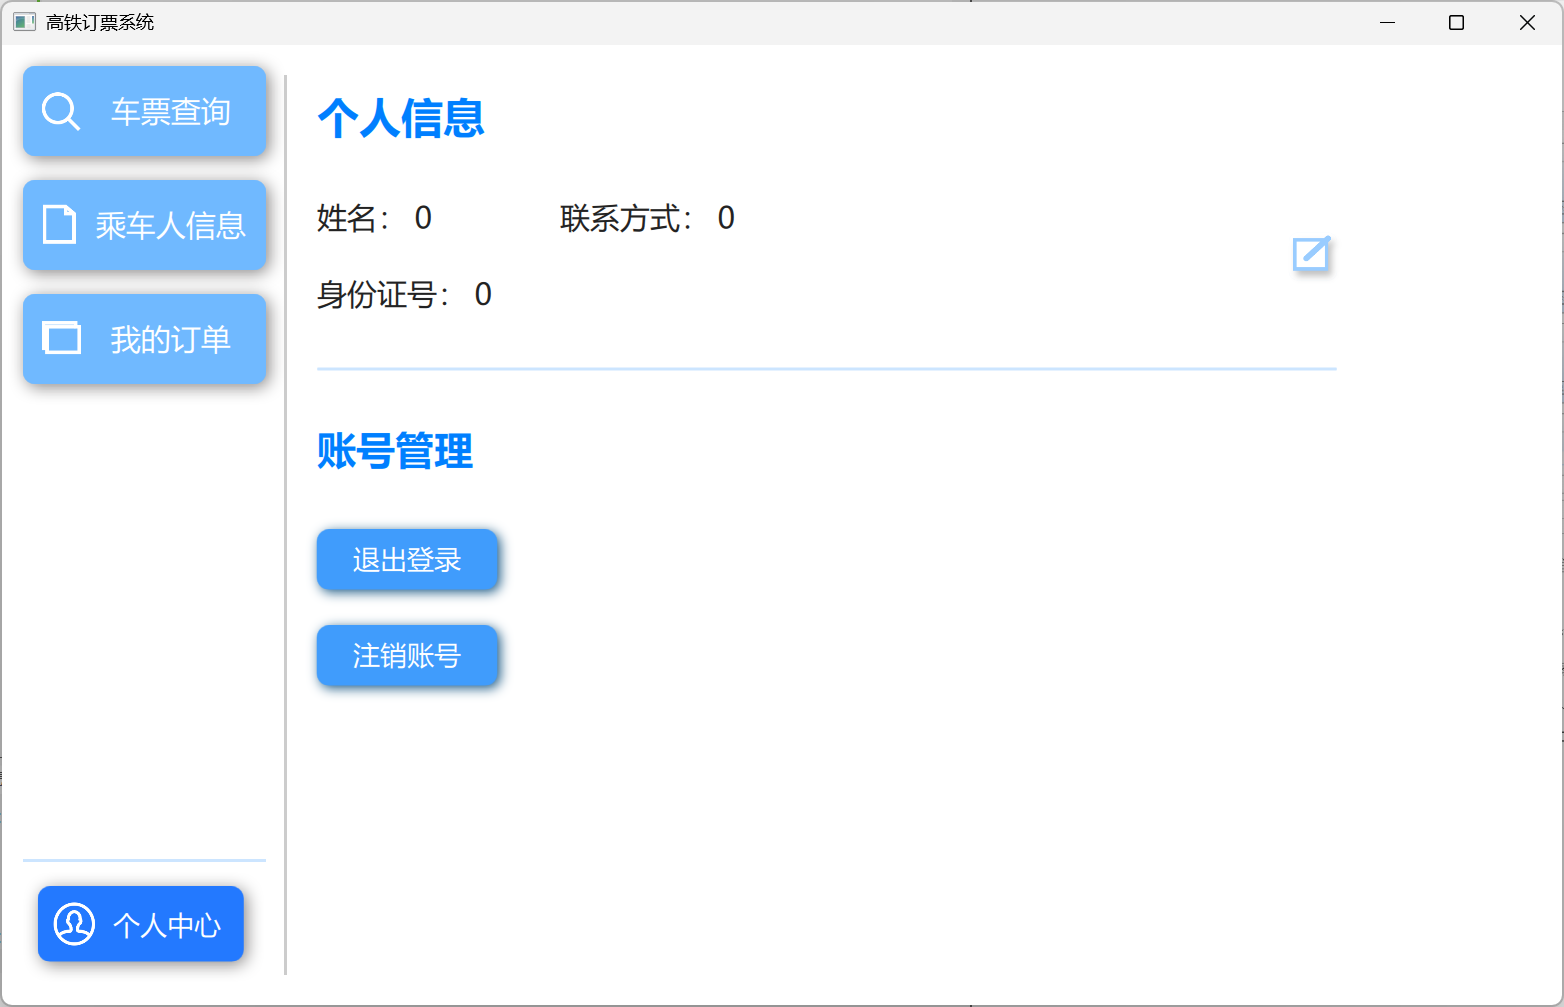
\includegraphics[width=0.7\textwidth]{个人信息修改与账号管理功能.png}
		\caption{个人信息修改与账号管理功能}
		\label{个人信息修改与账号管理功能}
	\end{figure}
	
	\paragraph{个人信息修改与账号管理功能}
	
	\paragraph{乘车人信息管理功能} 用户在侧边栏切换当前页面为“个人中心”，即可查看用户个人信息，如图\ref{个人信息修改与账号管理功能}所示。点击个人信息旁的修改图标，即可修改个人信息，包括姓名、身份证号和手机号。另外，点击下方的退出登录按钮，即可取消当前登录状态并返回到首页。点击注销账号按钮，即可注销当前账号并实现数据的级联删除（先删除用户所有订单和乘车人信息，再删除用户信息）。
	
	\subsubsection{管理员功能}
	\begin{figure}[H]
		\centering
		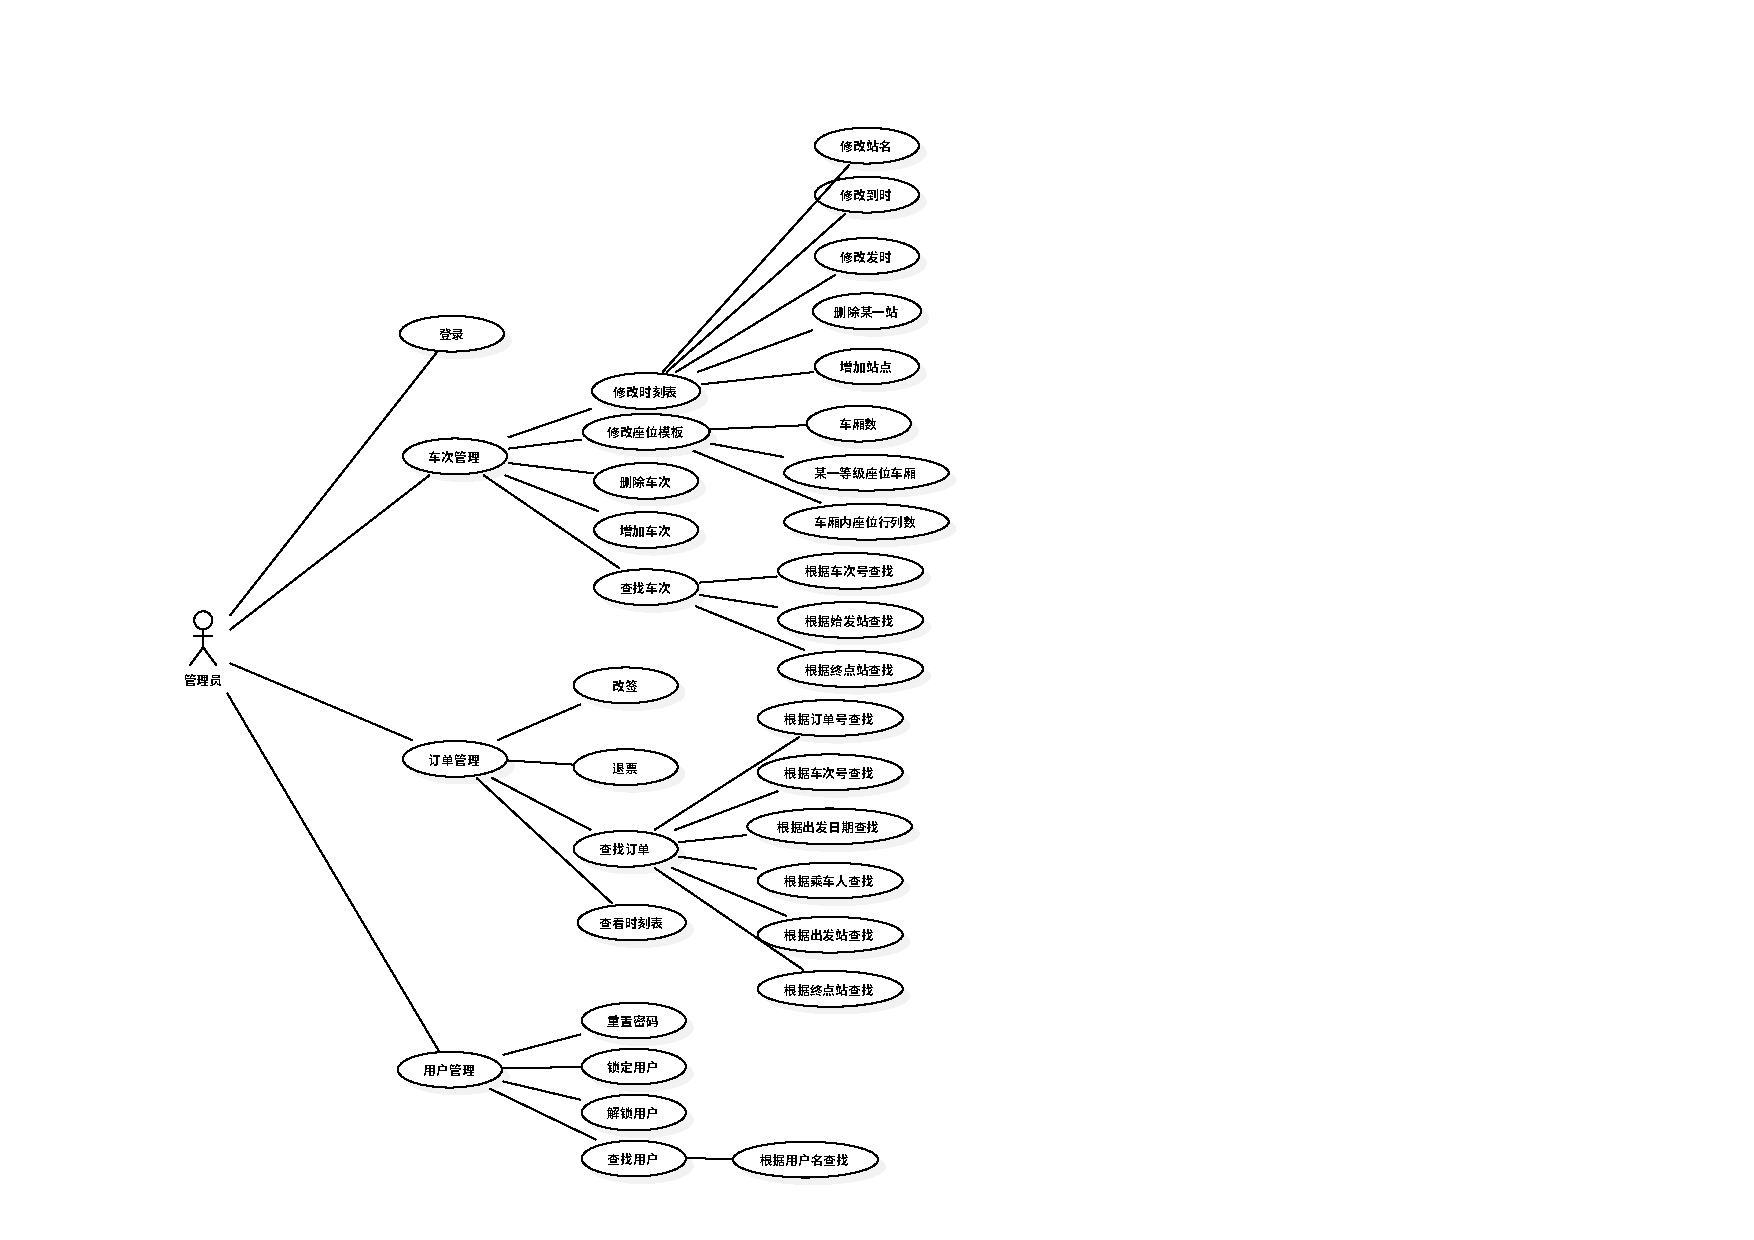
\includegraphics[width=1.5\textwidth]{管理员用例图.pdf}
		\caption{管理员用例图}
	\end{figure}
	
	管理员负责系统的后台维护与运营管理，需先完成登录后进入管理端。管理员主要围绕车次资源、订单业务与用户账户三方面开展工作：在车次管理中，可对车次信息进行增删改查，并对列车时刻表及座位模板等关键配置进行维护，以保证车次数据的准确性与可用性；在订单管理中，可对订单进行查询与处理，支持退票、改签等业务操作，并可查看关联时刻信息以辅助核对；在用户管理中，可对用户账户进行查询与维护，包括重置密码、锁定与解锁用户等，从而保障系统运行安全与业务秩序。以下是一些主要功能的详细介绍（\textbf{界面图片与前期设想和手工绘制一致}）。
	
	\begin{figure}[H]
		\centering
		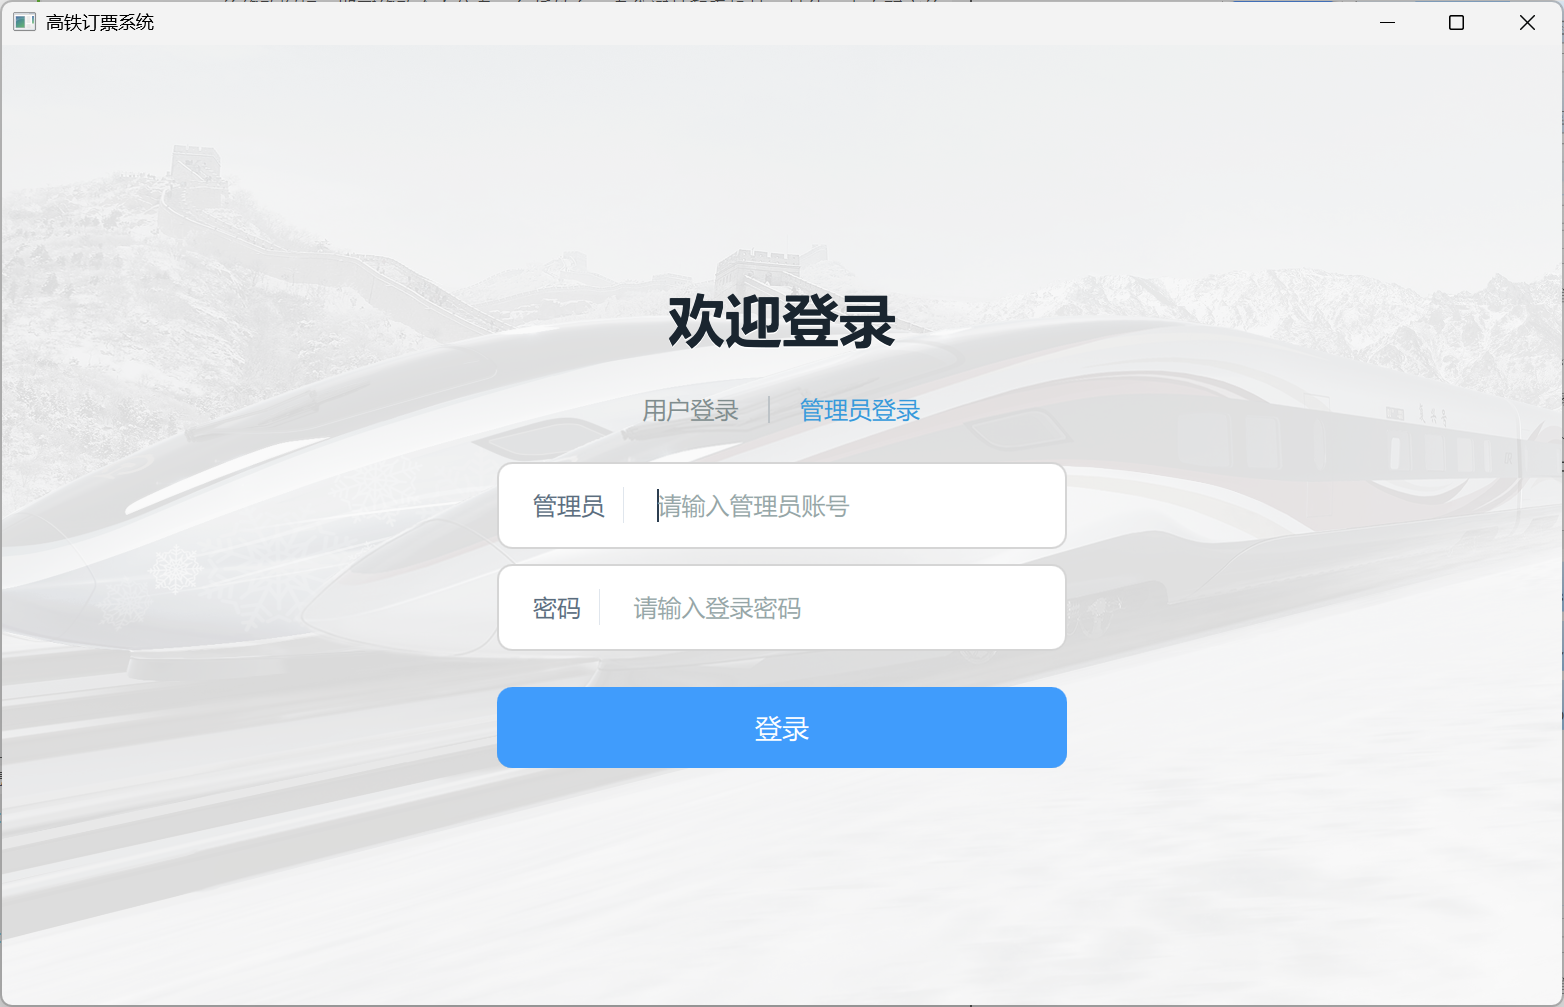
\includegraphics[width=0.7\textwidth]{管理员登录功能.png}
		\caption{管理员登录功能}
		\label{管理员登录功能}
	\end{figure}
	
	\paragraph{登录} 如图\ref{管理员登录功能}所示，管理员在登录界面点击“管理员登录”，通过在输入框中输入用户名和密码，点击登录后能够进行登录操作。如果用户名和密码正确，则登录成功，进入首页；否则系统会以弹窗提示的形式告诉管理员出现的问题，由管理员进行修改。
	
	\begin{figure}[H]
		\centering
		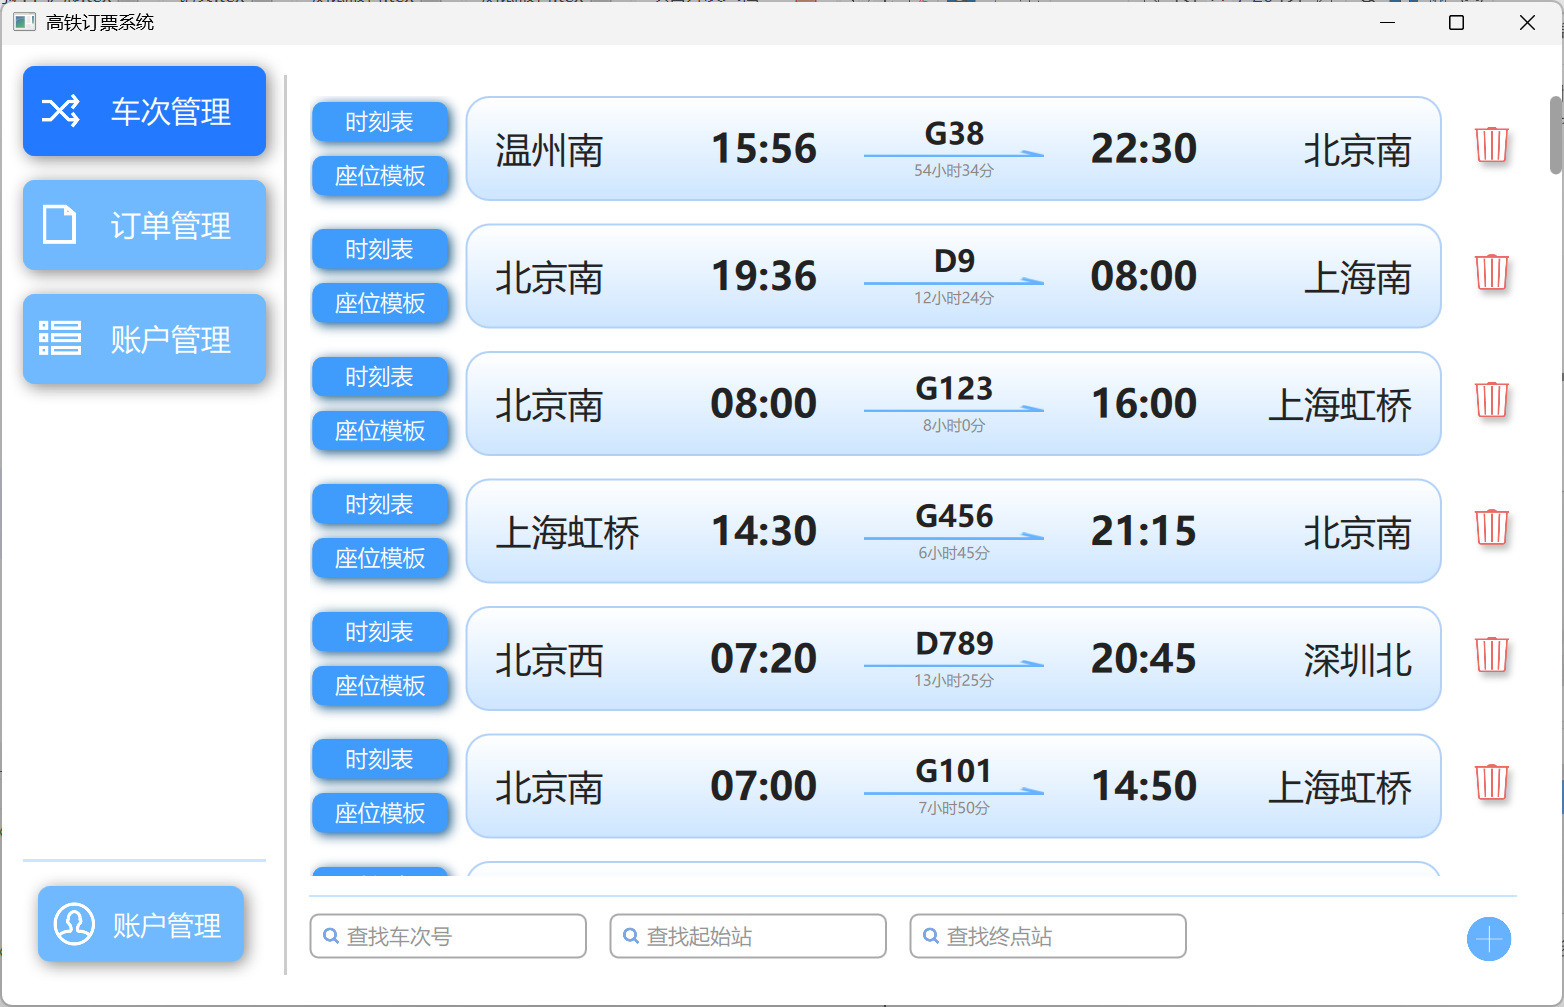
\includegraphics[width=0.7\textwidth]{车次管理功能.png}
		\caption{车次管理功能}
		\label{车次管理功能}
	\end{figure}
	
	\begin{figure}[H]
		\centering
		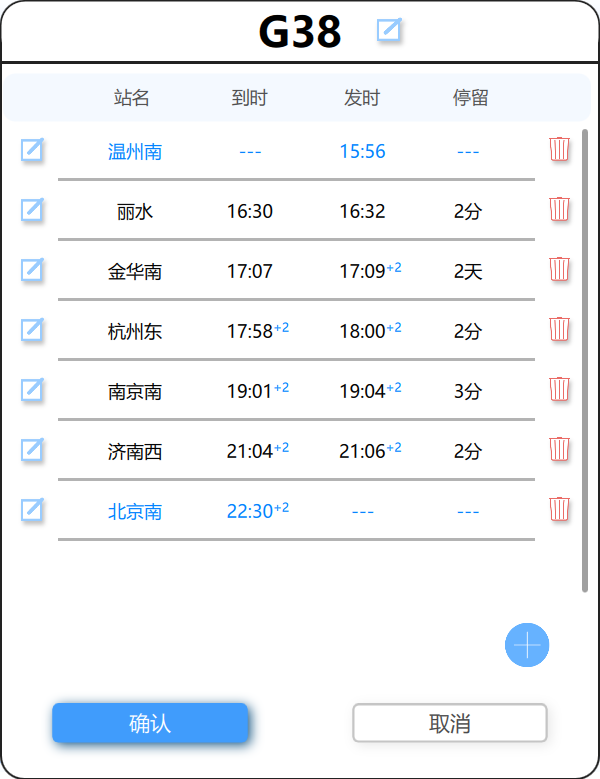
\includegraphics[width=0.4\textwidth]{修改时刻表功能.png}
		\caption{修改时刻表功能}
		\label{修改时刻表功能}
	\end{figure}
	
	\begin{figure}[H]
		\centering
		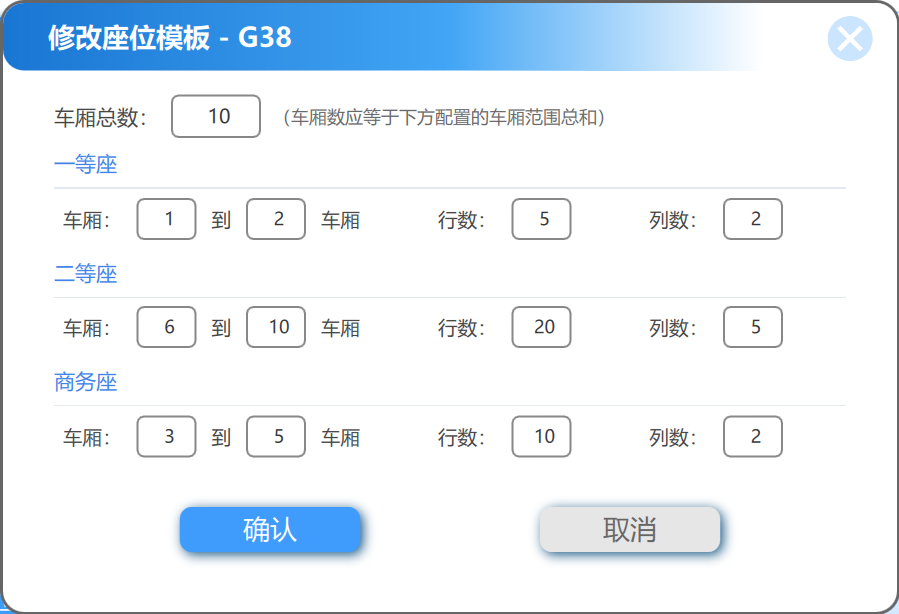
\includegraphics[width=0.5\textwidth]{修改座位模板功能.png}
		\caption{修改座位模板功能}
		\label{修改座位模板功能}
	\end{figure}
	
	\paragraph{车次管理功能} 管理员登录后，系统自动进入“车次管理”界面，如图\ref{车次管理功能}所示。管理员可在该页面查看和管理所有车次。在最下方的搜索框中可以对车次进行某些字段的搜素（支持多条件搜索）。点击右下角的加号，即可添加新的车次信息。点击对应车次的删除按钮，即可删除对应车次。系统应提供修改时刻表和座位模板功能，点击按钮后弹出的界面如图\ref{修改时刻表功能}和\ref{修改座位模板功能}所示。在修改时刻表界面，管理员能够添加、修改、删除各个停靠站，还可以修改车次名；在修改座位模板界面，管理员能够调整车箱数、每个车厢的座位等级和行列数。
	
	\begin{figure}[H]
		\centering
		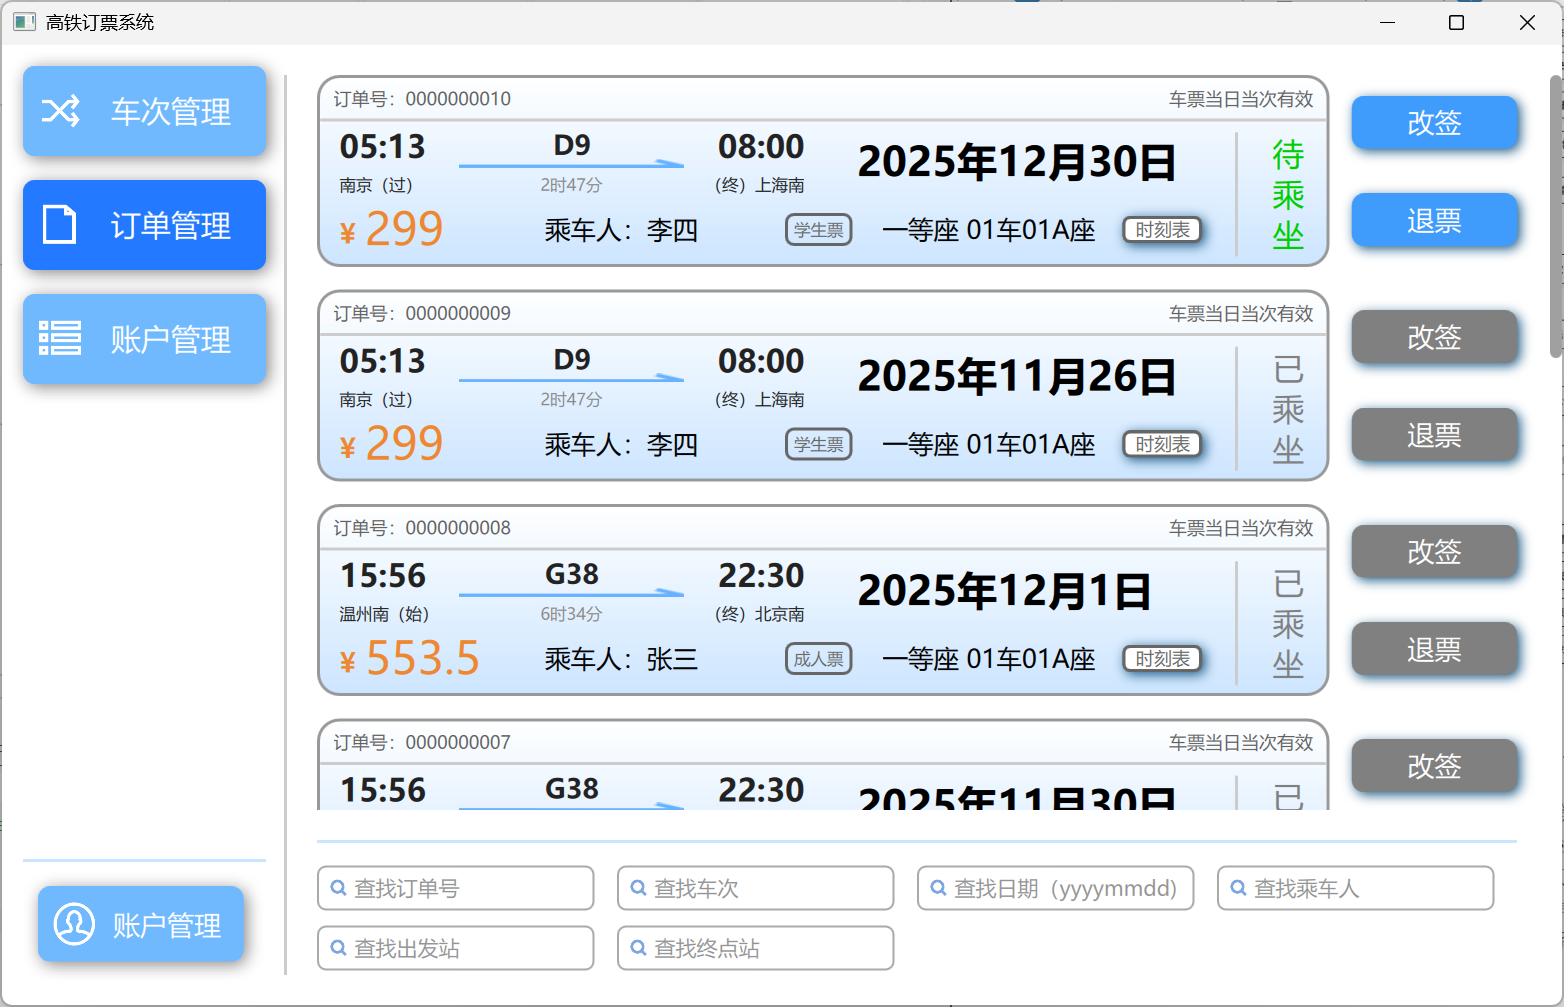
\includegraphics[width=0.7\textwidth]{管理员订单管理功能.png}
		\caption{管理员订单管理功能}
		\label{管理员订单管理功能}
	\end{figure}
	
	\paragraph{订单管理功能} 管理员点击侧边栏的“订单管理”即可切换到订单管理界面，如图\ref{管理员订单管理功能}所示。系统所提供的功能和提供给用户的“我的订单”功能基本一致，这里不再赘述。
	
	\begin{figure}[H]
		\centering
		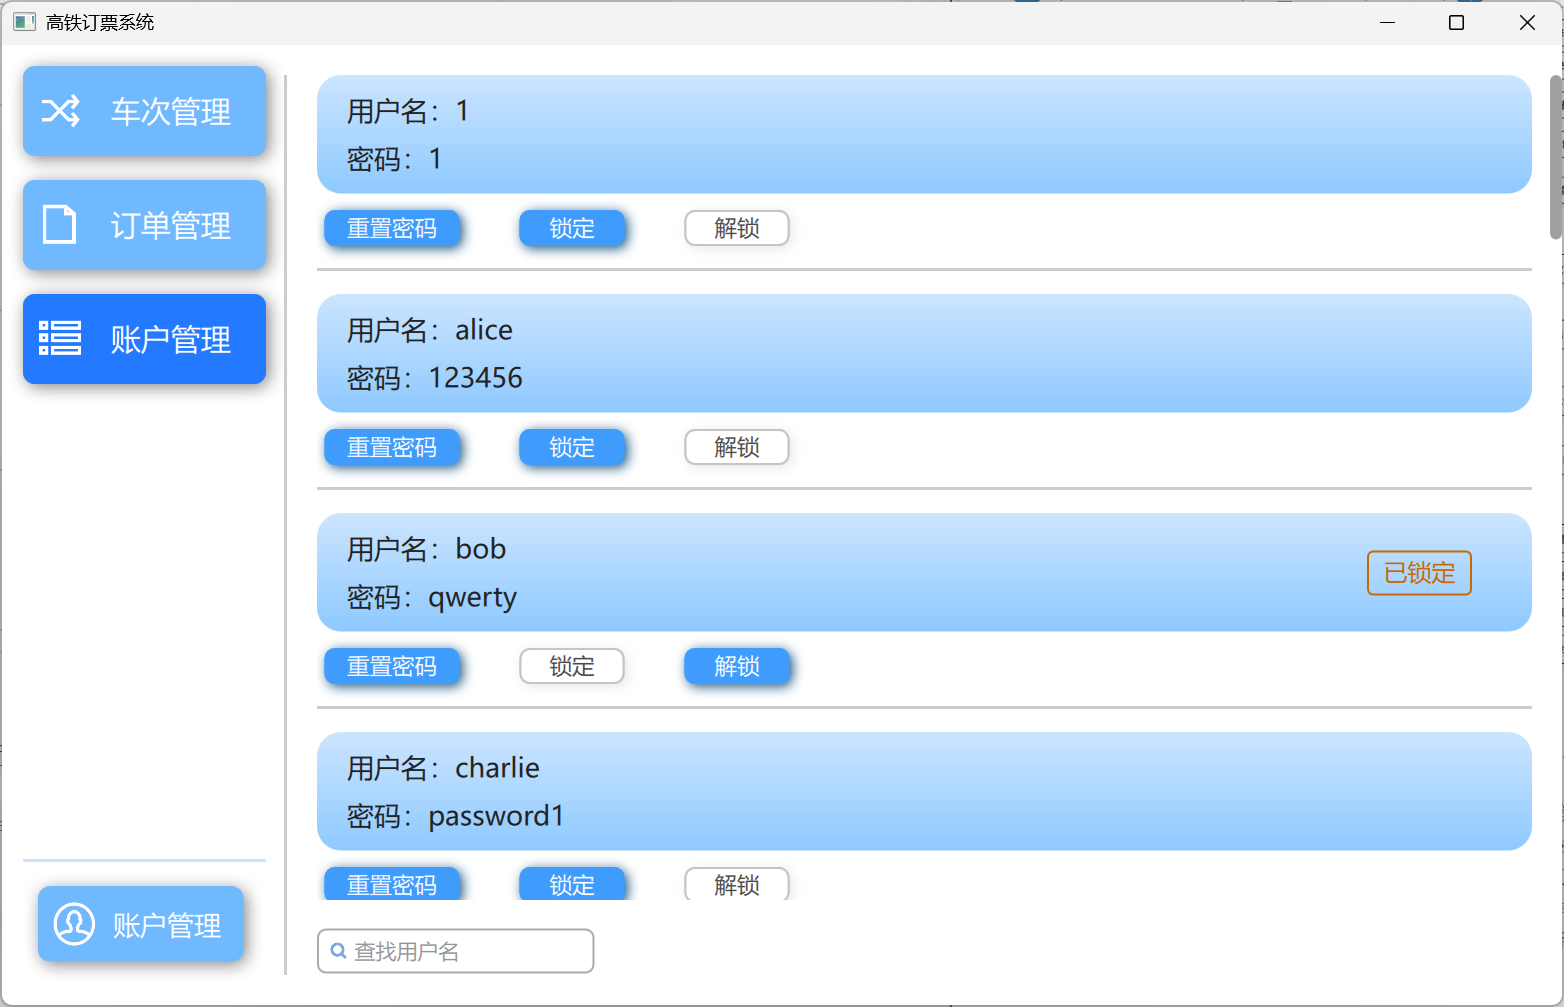
\includegraphics[width=0.7\textwidth]{账户管理功能.png}
		\caption{账户管理功能}
		\label{账户管理功能}
	\end{figure}
	
	\paragraph{账户管理功能} 管理员点击侧边栏的“账户管理”即可切换到账户管理界面，如图\ref{账户管理功能}所示。系统应提供对每个账户（用户和其他管理员）的重置密码、锁定和解锁功能。同时，管理员在最下方的搜索框搜索用户名，即可显示模糊匹配成功的账户信息。
	
	\subsubsection{通用功能}
	通用功能为系统提供给所有账户角色的功能，在本系统中，用户和管理员都能使用的功能。主要功能如下：
	
	\begin{figure}[H]
		\centering
		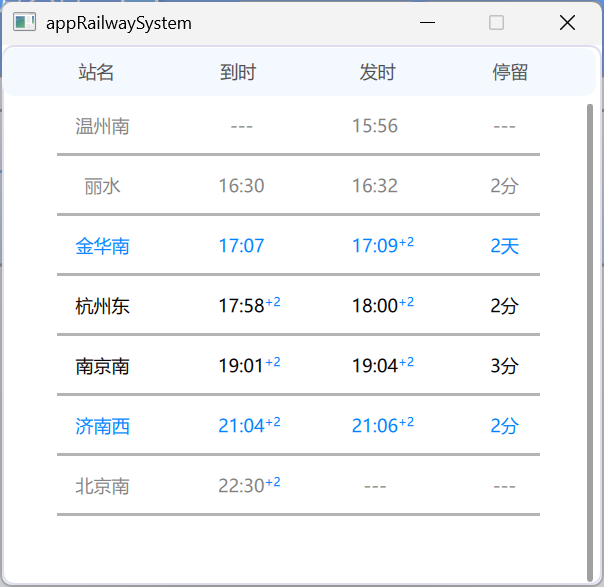
\includegraphics[width=0.4\textwidth]{查看时刻表功能.png}
		\caption{查看时刻表功能}
		\label{查看时刻表功能}
	\end{figure}
	
	\paragraph{查看订单/车次/余票的时刻表} 用户在“我的订单”和车票查询结果界面，以及最终的确认订单界面，均可以点击“时刻表”按钮查看对应车次的时刻表；管理员同样可以点击查看车次或者订单的时刻表。时刻表表面应如图\ref{查看时刻表功能}所示，显示每个停靠站的站名、到时、发时和停留时间。对于订单的时刻表，存在起末站，系统应将起末站标蓝色，停靠站标灰色而处于订单停靠区间外的停靠站标灰色，便于用户和管理员查看。另外，还应以数字角标的方式提示用户停靠站的到时或发时是否是当天还是第二天或第三天等（考虑过夜、隔天的车次）。
	
	\begin{figure}[H]
		\centering
		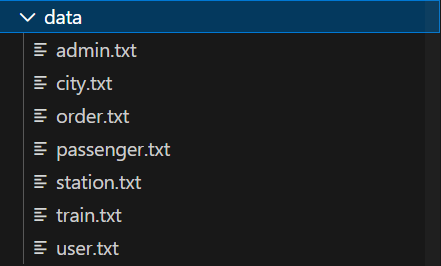
\includegraphics[width=0.4\textwidth]{数据文件.png}
		\caption{数据文件}
		\label{数据文件}
	\end{figure}
	
	\paragraph{数据装载与保存} 本系统所有数据全部以txt形式存储在\texttt{data/}目录下，如图\ref{数据文件}所示，包括以下几个文件：
	
	\begin{itemize}
		\item \texttt{admin.txt}：存储所有管理员的用户名和密码等
		\item \texttt{user.txt}：存储所有用户的用户名、密码和个人信息等
		\item \texttt{passenger.txt}：存储所有用户的所有乘车人信息，用户名和身份证作为主码唯一确定一条乘车人信息
		\item \texttt{order.txt}：存储所有用户的所有订单信息，包括日期、座位等级、座位号、车次、起末站、时刻表等信息，订单号作为主码唯一确定一条订单信息
		\item \texttt{train.txt}：存储所有车次信息，包括起末站、时刻表、座位模板等信息，车次号作为主码唯一确定一条车次信息
		\item \texttt{station.txt}：存储所有车站的车站名和所处城市
		\item \texttt{city.txt}：存储所有城市的城市名和经纬度（\textbf{只读}），经纬度用于计算距离和票价
	\end{itemize}
	
	程序启动时，各个类对象执行构造函数时读取各自需要的信息装入内存，待用户操作完毕关闭程序时，由析构函数完成数据的保存和持久化。
	
	
	\subsection{非功能性需求}
	\subsubsection{可维护性}
	系统在设计上应遵循模块化与低耦合原则，将用户端、管理端、车次/时刻、订单、乘车人、权限认证等功能划分为相对独立的模块，各模块职责单一、边界清晰。通过统一的接口与公共组件复用降低重复代码与修改成本，确保当业务规则或页面逻辑发生调整时，能够在局部范围内完成修改并快速定位问题，从而提升系统的长期维护效率。
	
	\subsubsection{可扩展性}
	系统需具备良好的扩展空间，以适应业务增长与规则变化。在数据模型与业务逻辑层面，应支持灵活新增车次、站点与时刻信息，并允许在不破坏既有功能的前提下引入新的筛选/排序维度、票价与座席规则、订单处理策略等。整体架构应尽量采用可配置、可插拔的方式组织规则与参数，降低新增功能对核心流程的侵入性。
	
	\subsubsection{易用性}
	系统界面与交互应以用户任务为导向，保证信息层级清晰、页面布局简洁，关键操作入口明确且一致。常用流程（如查询、订票、订单管理）应减少不必要的步骤，操作路径短且可预期；对用户输入提供必要的提示、校验与错误反馈，使用户能够在较低学习成本下完成主要功能，提高使用效率与满意度。
	
	\subsubsection{数据安全性}
	系统应对不同角色与不同操作范围进行权限区分，确保普通用户与管理员仅能访问各自授权的功能与数据；对涉及敏感信息的操作应进行身份校验与必要的二次确认。账户安全方面应提供账户锁定机制（例如多次登录失败后限制登录）以及密码重置等能力，以降低暴力破解与越权访问风险。同时，系统应保障关键业务数据的完整性与一致性，避免因异常操作导致数据被非法篡改或错误更新。
	
	\section{系统总体设计}
	\subsection{系统架构}
	本系统采用基于 MVC 的界面与逻辑分离设计，使用 C++、QML和Javascript 实现：QML 负责界面展示与交互，Javascript负责前端逻辑，C++ 负责业务处理与数据管理。整体思路是在桌面端实现“界面做界面、逻辑做逻辑”，减少相互影响，便于后续修改与迭代。
	
	系统按层次划分为三部分：界面层负责页面显示与用户操作；中间层负责接收界面事件并调用相应功能；数据与业务层负责具体规则处理以及数据读写。界面层不直接处理复杂规则，只通过接口获取结果并展示，从而让界面保持简洁清晰。
	
	在模块划分上，系统以 Manager 的方式组织功能：每个 Manager 只负责一类任务，例如车次与时刻、订单、用户与权限等，并对外提供统一的调用入口。通过这种划分方式，各模块边界明确，修改某一功能时更容易定位，且便于后续增加新车次、新规则等扩展需求。
	
	\subsection{代码规范}
	为了实现系统非功能性需求，保证代码可读、可维护性，良好、规范、易理解的代码规范能够大大提高开发效率并确保系统可维护性的提高，高铁管理系统在代码编写过程中必须遵循一系列严格的规范：
	\begin{itemize}
		\item 文件和目录组织：将QML页面文件集中放在pages/目录下、组件文件放在components/目录下、后端C++类文件按功能分组（如Manager类负责数据管理、实体类如User和Train封装数据模型）。所有QML文件、C++源文件（.cpp）和C++头文件（.h）全部以帕斯卡命名法（单词首字母大写）命名
		\item 代码标识符命名：
		\begin{itemize}
			\item 类的属性：小写字母+下划线命名
			\item 类的普通方法：驼峰命名法
			\item 类暴露给前端的接口：驼峰命名法+\_api后缀
			\item 局部变量：驼峰命名法
			\item JS变量和函数：驼峰命名法
		\end{itemize}
		\item 注释风格：使用中文注释解释关键逻辑，如函数头部注释“// 获取所有城市名称”，行内注释简洁明了
		\item 错误处理：使用 \texttt{QVariantMap} 返回结果，包含 \texttt{success} 和 \texttt{message} 字段，便于前端处理
	\end{itemize}
	
	\subsection{类的静态设计}
	\subsubsection{基本实体类}
	
	\begin{figure}[H]
		\centering
		\includesvg{Time.svg}
		\caption{Time}
		\label{Time}
	\end{figure}
	
	\begin{lstlisting}[language=C++, caption={Time}]
		#ifndef TIME_H
		#define TIME_H
		#include <iostream>
		
		class Time
		{
			private:
			int hour = -1;
			int minute = -1;
			int second = -1;
			
			public:
			Time();
			Time(int hour, int minute, int second=0);
			
			int getHour();
			bool setHour(int hour);
			int getMinute();
			bool setMinute(int minute);
			int getSecond();
			bool setSecond(int second);
			bool isNull();
			bool setNull();
			
			bool now();
			
			friend bool operator==(const Time &t1, const Time &t2);
			friend bool operator!=(const Time &t1, const Time &t2);
			friend int operator-(const Time &t1, const Time &t2);
			friend bool operator<(const Time &t1, const Time &t2);
			friend std::ostream &operator<<(std::ostream &os, Time &t);
			friend std::istream &operator>>(std::istream &is, Time &t);
		};
		
		#endif // TIME_H\end{lstlisting}
	
	\paragraph{\texttt{Time}：时间类} 负责维护某个时间信息，包含整型存储的时、分、秒属性，以及基本的getter、setter和运算符重载方法。此外，还包含\texttt{now()}方法，用以设置当前时间对象为系统实际时间。
	
	
	\begin{figure}[H]
		\centering
		\includesvg{Date.svg}
		\caption{Date}
		\label{Date}
	\end{figure}
	
	\begin{lstlisting}[language=C++, caption={Date}]
		#ifndef DATE_H
		#define DATE_H
		#include <iostream>
		
		class Date
		{
			private:
			int year = -1;
			int month = -1;
			int day = -1;
			
			public:
			Date();
			Date(int year, int month, int day);
			int getYear();
			bool setYear(int year);
			int getMonth();
			bool setMonth(int month);
			int getDay();
			bool setDay(int day);
			
			bool now();
			
			friend Date operator+(const Date &d, int days);
			friend Date operator-(const Date &d, int days);
			friend int operator-(const Date &d1, const Date &d2);
			friend bool operator<(const Date &d1, const Date &d2);
			friend bool operator>(const Date &d1, const Date &d2);
			friend bool operator>=(const Date &d1, const Date &d2);
			friend bool operator<=(const Date &d1, const Date &d2);
			friend bool operator==(const Date &d1, const Date &d2);
			friend bool operator!=(const Date &d1, const Date &d2);
			friend std::ostream &operator<<(std::ostream &os, const Date &d);
			friend std::istream &operator>>(std::istream &is, Date &d);
		};
		
		#endif // DATE_H\end{lstlisting}
	
	\paragraph{\texttt{Date}：日期类} 日期类负责维护一个日期信息，包含整型存储的年月日属性，以及若干getter、setter方法和运算符重载。此外，还包含\texttt{now()}方法，用以设置当前日期对象为系统实际日期。
	
	\begin{figure}[H]
		\centering
		\includesvg{UserProfile.svg}
		\caption{UserProfile}
		\label{UserProfile}
	\end{figure}
	
	\begin{lstlisting}[language=C++, caption={UserProfile}]
		#ifndef USERPROFILE_H
		#define USERPROFILE_H
		#include <QString>
		
		class UserProfile
		{
			private:
			QString name = "";
			QString phone_number = "";
			QString id = "";
			
			public:
			UserProfile();
			UserProfile(const QString &name,
			const QString &phone_number,
			const QString &id);
			
			QString getName();
			bool setName(const QString &name);
			QString getPhoneNumber();
			bool setPhoneNumber(const QString &phone_number);
			QString getId();
			bool setId(const QString &id);
			
			friend bool operator==(const UserProfile &up1, const UserProfile &up2);
			friend bool operator!=(const UserProfile &up1, const UserProfile &up2);
			friend std::istream& operator>>(std::istream& is, UserProfile& up);
			friend std::ostream& operator<<(std::ostream& os, const UserProfile& up);
		};
		
		#endif // USERPROFILE_H\end{lstlisting}
	
	\paragraph{\texttt{UserProfile}：用户个人信息类} 负责维护用户个人信息，包含姓名、手机号、身份证号等属性和基本的getter、setter和运算符重载方法。
	
	\begin{figure}[H]
		\centering
		\includesvg{User.svg}
		\caption{User}
		\label{User}
	\end{figure}
	
	\begin{lstlisting}[language=C++, caption={User}]
		#ifndef USER_H
		#define USER_H
		#include <QString>
		#include "userprofile.h"
		
		class User
		{
			private:
			UserProfile profile;
			bool locked = false;
			QString username = "";
			QString password = "";
			
			public:
			User();
			User(UserProfile &profile, bool locked, const QString &username, const QString &password);
			
			UserProfile getProfile();
			bool setProfile(const UserProfile &profile);
			bool isLocked();
			bool lock();
			bool unlock();
			QString getUsername();
			bool setUsername(const QString &username);
			QString getPassword();
			bool setPassword(const QString &password);
			
			User& operator()(const UserProfile &profile, bool locked, const QString &username, const QString &password);
			friend bool operator==(const User &u1, const User &u2);
			friend bool operator!=(const User &u1, const User &u2);
			friend std::istream& operator>>(std::istream& is, User& u);
			friend std::ostream& operator<<(std::ostream& os, const User& u);
		};
		
		#endif // USER_H\end{lstlisting}
	
	\paragraph{\texttt{User}：用户类} 负责维护用户信息，包含用户名、密码、用户个人信息和锁定状态等属性，以及基本的getter、setter和运算符重载方法。
	
	\begin{figure}[H]
		\centering
		\includesvg{Admin.svg}
		\caption{Admin}
		\label{Admin}
	\end{figure}
	
	\begin{lstlisting}[language=C++, caption={Admin}]
		#ifndef ADMIN_H
		#define ADMIN_H
		#include <QString>
		
		class Admin
		{
			private:
			QString username = "";
			QString password = "";
			bool locked = false;
			public:
			Admin();
			
			QString getUsername();
			bool setUsername(const QString &username);
			QString getPassword();
			bool setPassword(const QString &password);
			bool isLocked();
			bool lock();
			bool unlock();
			
			Admin& operator()(const QString &username, const QString &password, bool locked);
			friend bool operator==(const Admin &a1, const Admin &a2);
			friend bool operator!=(const Admin &a1, const Admin &a2);
			friend std::istream& operator>>(std::istream& is, Admin& a);
			friend std::ostream& operator<<(std::ostream& os, const Admin& a);
		};
		
		#endif // ADMIN_H\end{lstlisting}
	
	\paragraph{\texttt{Admin}：管理员类} 负责维护管理员信息，包括用户名、密码和锁定状态属性，以及基本的getter、setter和运算符重载方法。
	
	\begin{figure}[H]
		\centering
		\includesvg{Passenger.svg}
		\caption{Passenger}
		\label{Passenger}
	\end{figure}
	
	\begin{lstlisting}[language=C++, caption={Passenger}]
		#ifndef PASSENGER_H
		#define PASSENGER_H
		#include <QString>
		#include <iostream>
		
		class Passenger
		{
			private:
			QString name = "";
			QString phone_number = "";
			QString id = "";
			QString type = "";
			QString username = "";
			
			public:
			Passenger();
			Passenger(const QString &name, const QString &phoneNumber,
			const QString &id, const QString &type, const QString &username);
			
			QString getName();
			bool setName(const QString &name);
			QString getPhoneNumber();
			bool setPhoneNumber(const QString &phone);
			QString getId();
			bool setId(const QString &id);
			QString getType();
			bool setType(const QString &type);
			QString getUsername();
			bool setUsername(const QString &username);
			
			friend bool operator==(const Passenger &p1, const Passenger &p2);
			friend bool operator!=(const Passenger &p1, const Passenger &p2);
			friend std::ostream &operator<<(std::ostream &os, const Passenger &p);
			friend std::istream &operator>>(std::istream &is, Passenger &p);
		};
		
		#endif // PASSENGER_H\end{lstlisting}
	
	\paragraph{\texttt{Passenger}：乘车人类} 负责维护一个乘车人的信息，包括姓名、手机号、身份证（儿童/学生/成人）、用户名（所属用户）属性以及基本的getter、setter和运算符重载方法。
	
	\begin{figure}[H]
		\centering
		\includesvg{Station.svg}
		\caption{Station}
		\label{Station}
	\end{figure}
	
	\begin{lstlisting}[language=C++, caption={Station}]
		#ifndef STATION_H
		#define STATION_H
		#include <vector>
		#include "city.h"
		
		class Station
		{
			private:
			QString station_name = "";
			QString city_name = "";
			
			public:
			Station();
			Station(const QString &stationName, const QString &cityName);
			
			QString getStationName();
			QString getCityName();
			bool setStationName(const QString &name);
			bool setCityName(const QString &name);
			
			friend bool operator==(const Station &s1, const Station &s2);
			friend bool operator!=(const Station &s1, const Station &s2);
			friend std::istream& operator>>(std::istream& is, Station& s);
			friend std::ostream& operator<<(std::ostream& os, const Station& s);
		};
		
		#endif // STATION_H\end{lstlisting}
	
	\paragraph{\texttt{Station}：车站类} 负责维护一个车站的信息，包括车站名和所属城市名以及基本的getter、setter和运算符重载方法。
	
	\begin{figure}[H]
		\centering
		\includesvg{City.svg}
		\caption{City}
		\label{City}
	\end{figure}
	
	\begin{lstlisting}[language=C++, caption={City}]
		#ifndef CITY_H
		#define CITY_H
		
		#include <QString>
		
		class City
		{
			private:
			QString name = "";
			double longitude;
			double latitude;
			QString province = "";
			public:
			City();
			
			QString getName();
			double getLongitude();
			double getLatitude();
			QString getProvince();
			
			friend bool operator==(const City &c1, const City &c2);
			friend bool operator!=(const City &c1, const City &c2);
			friend std::istream& operator>>(std::istream& is, City& c);
			friend std::ostream& operator<<(std::ostream& os, const City& c);
		};
		
		#endif // CITY_H\end{lstlisting}
	
	\paragraph{\texttt{City}：城市类} 负责维护一个城市的信息，包括城市名、经度、维度和所属省份以及基本的getter、setter和运算符重载方法。
	
	\begin{figure}[H]
		\centering
		\includesvg[width=\textwidth]{Timetable.svg}
		\caption{Timetable}
		\label{Timetable}
	\end{figure}
	
	\begin{lstlisting}[language=C++, caption={Timetable}]
		#ifndef TIMETABLE_H
		#define TIMETABLE_H
		#include "station.h"
		#include "time.h"
		#include <vector>
		#include <tuple>
		#include <iostream>
		
		class Timetable
		{
			private:
			std::vector<std::tuple<Station, Time, Time, int, int>> table;
			
			public:
			Timetable();
			
			// 输入某个车站，输出这个车站的信息（到时、发时、到天、发天、始/终/过）
			std::tuple<Time, Time, int, int, QString> getStationInfo(const QString &stationName);
			// 获得两个车站的时间间隔
			int getInterval(Station &station1, Station &station2);
			// 输入城市A和城市B，输出这个时刻表从A到B的所有车站组合
			std::vector<std::tuple<Station, Station>> getStationPairsBetweenCities(const QString &startCityName, const QString &endCityName);
			// 获得某个车站的索引（第几个停靠站）
			int getIndexByStationName(const QString &stationName);
			// 输出车站A和车站B，输出A到B经过的所有车站（包括A和B）
			std::vector<Station> getStationsBetweenStations(const Station &startStation, const Station &endStation);
			// 获得从起始站到终点站，中间每一站的信息（站，到时，发时，到达天数，发时天数，停留时间，起末站/中间站/其他站）
			std::vector<std::tuple<Station, Time, Time, int, int, int, QString>> getInfo(const QString &startStationName, const QString &endStationName);
			// 获得从起始站到终点站，中间每一站的信息（站，到时，发时，到达天数，发时天数，停留时间，起末站/中间站/其他站）重载函数
			std::vector<std::tuple<Station, Time, Time, int, int, int, QString>> getInfo();
			// 获得时刻表第一个车站的信息（站，发时）
			std::tuple<Station, Time> getStartStationInfo();
			// 获得时刻表最后一个车站的信息（站，到时）
			std::tuple<Station, Time> getEndStationInfo();
			// 在尾部插入一个停靠站
			bool insertPassingStationAtEnd(Station &station, Time &arriveTime, Time &departureTime, int arriveDay, int departureDay);
			
			friend bool operator==(const Timetable &t1, const Timetable &t2);
			friend bool operator!=(const Timetable &t1, const Timetable &t2);
			friend std::ostream &operator<<(std::ostream &os, Timetable &timetable);
			friend std::istream &operator>>(std::istream &is, Timetable &timetable);
		};
		
		#endif // TIMETABLE_H\end{lstlisting}
	
	\paragraph{\texttt{Timetable}：时刻表类} 负责维护一个时刻表的信息，属性包括一个元组动态数组，数组每个元素为一个五元组，分别为车站对象、到时、发时、到天（距离出发日期的偏移量）、发天（距离出发日期的偏移量），由若干五元组组成了整个时刻表。时刻表类除了运算符重载方法，还提供了多种多样的方法用于获取、查询、插入、删除等操作，具体功能可参考注释。
	
	\begin{figure}[H]
		\centering
		\includesvg{Train.svg}
		\caption{Train}
		\label{Train}
	\end{figure}
	
	\begin{lstlisting}[language=C++, caption={Train}]
		#ifndef TRAIN_H
		#define TRAIN_H
		#include <QString>
		#include "timetable.h"
		#include <vector>
		#include <tuple>
		
		class Train
		{
			private:
			QString number;
			Timetable timetable;
			std::vector<std::tuple<QString, int, int>> carriages;
			
			public:
			Train();
			
			QString getNumber();
			bool setNumber(const QString &number);
			Timetable getTimetable();
			bool setTimetable(Timetable &timetable);
			std::vector<std::tuple<QString, int, int>> getCarriages();
			bool setCarriages(std::vector<std::tuple<QString, int, int>> carriages);
			int getFirstClassCount();
			int getSecondClassCount();
			int getBusinessClassCount();
			
			friend bool operator==(const Train &t1, const Train &t2);
			friend bool operator!=(const Train &t1, const Train &t2);
			
			friend std::istream &operator>>(std::istream &is, Train &train);
			friend std::ostream &operator<<(std::ostream &os, Train &train);
		};
		
		#endif // TRAIN_H\end{lstlisting}
	
	\paragraph{\texttt{Train}：车次类} 负责维护一个车次的信息，包含订单号、时刻表属性，以及carriages属性。carriages也是一个元组动态数组，数组每个元素对应一个车厢，由一个三元组表示，分别代表座位等级（二等座/一等座/商务座）、座位行数、座位列数。该类除了基本的getter、setter和运算符重载方法，还提供了\texttt{get-XXX-count()}方法用于获取各个座位等级的座位数量。
	
	\begin{figure}[H]
		\centering
		\includesvg[width=\textwidth]{Order.svg}
		\caption{Order}
		\label{Order}
	\end{figure}
	
	\begin{lstlisting}[language=C++, caption={Order}]
		#ifndef ORDER_H
		#define ORDER_H
		#include <QString>
		#include "passenger.h"
		#include "timetable.h"
		#include "date.h"
		
		class Order
		{
			private:
			QString order_number = "";
			QString train_number = "";
			Passenger passenger;
			double price = -1;
			Date date;
			Station start_station;
			Station end_station;
			Timetable timetable;
			QString seat_level = "";
			int carriage_number = -1;
			int seat_row = -1;
			int seat_col = -1;
			QString status = "";
			QString username = "";
			
			public:
			Order();
			Order(const QString &orderNumber, const QString &trainNumber,
			const Passenger &passenger, double price, const Date &date,
			const Timetable &timetable, const Station &startStation,
			const Station &endStation, const QString &seatLevel,
			int carriageNumber, int seatRow, int seatCol,
			const QString &status, const QString &username);
			
			QString getOrderNumber();
			bool setOrderNumber(const QString &orderNumber);
			QString getTrainNumber();
			bool setTrainNumber(const QString &trainNumber);
			Passenger getPassenger();
			bool setPassenger(const Passenger &passenger);
			double getPrice();
			bool setPrice(double price);
			Date getDate();
			bool setDate(const Date &date);
			Station getStartStation();
			bool setStartStation(const Station &startStation);
			Station getEndStation();
			bool setEndStation(const Station &endStation);
			Timetable getTimetable();
			bool setTimetable(const Timetable &timetable);
			QString getSeatLevel();
			bool setSeatLevel(const QString &seatLevel);
			int getCarriageNumber();
			bool setCarriageNumber(int carriageNumber);
			int getSeatRow();
			bool setSeatRow(int seatRow);
			int getSeatCol();
			bool setSeatCol(int seatCol);
			QString getStatus();
			bool setStatus(const QString &status);
			QString getUsername();
			bool setUsername(const QString &username);
			
			Date getEndDate();
			Time getStartTime();
			Time getEndTime();
			bool isTimeRangeOverlap(Date &queryStartDate, Time &queryStartTime, Date &queryEndDate, Time &queryEndTime);
			
			friend bool operator==(const Order &o1, const Order &o2);
			friend bool operator!=(const Order &o1, const Order &o2);
			friend std::ostream &operator<<(std::ostream &os, Order &o);
			friend std::istream &operator>>(std::istream &is, Order &o);
		};
		
		#endif // ORDER_H\end{lstlisting}
	
	\paragraph{\texttt{Order}：订单类} 负责维护一个订单的信息，包括订单号、车次号、乘车人、订单价格、出发日期、始发站、终点站、时刻表、座位等级、车厢号、座位行号、座位列号、状态（已取消/待乘坐/已改签/已乘坐）等属性。除了基本的getter、setter和运算符重载函数，还提供\texttt{getStartDate}、\texttt{getEndDate}、\texttt{getEndTime}方法，用于获取出发日期、结束日期、结束时间（根据时刻表计算得到，无法直接通过订单属性获得）。另外，\texttt{isTimeRangeOverlap()}方法用于检测该订单的始末日期是否和传入的时间区间重叠。
	
	\subsubsection{数据管理类}
	数据管理类用于对上述实体进行同一管理和操作，并且兼具向前端提供接口的功能。所有数据管理类均继承自\texttt{QObject}，可以使用\texttt{Q\_INVOKABLE}宏修饰函数，表示该函数可被前端调用。
	
	\begin{figure}[H]
		\centering
		\includesvg[width=\textwidth]{AccountManager.svg}
		\caption{AccountManager}
		\label{AccountManager}
	\end{figure}
	
	\begin{lstlisting}[language=C++, caption={AccountManager}]
		#ifndef ACCOUNTMANAGER_H
		#define ACCOUNTMANAGER_H
		
		#include <QObject>
		#include <QVariantList>
		#include <QVariantMap>
		#include <vector>
		#include "user.h"
		#include "admin.h"
		
		class AccountManager : public QObject
		{
			Q_OBJECT
			
			public:
			std::vector<User> users;
			std::vector<Admin> admins;
			
			public:
			explicit AccountManager(QObject *parent = nullptr);
			
			// 用户登录
			Q_INVOKABLE QVariantMap loginUser_api(const QString &username, const QString &password);
			// 管理员登录
			Q_INVOKABLE QVariantMap loginAdmin_api(const QString &username, const QString &password);
			// 获取用户个人信息，传入用户名
			Q_INVOKABLE QVariantMap getUserProfile_api(const QString &username);
			// 获取所有账户信息，返回账户列表
			Q_INVOKABLE QVariantList getAccounts_api();
			// 对某个用户加锁，传入用户名
			Q_INVOKABLE QVariantMap lockUser_api(const QString &username);
			// 对某个管理员加锁，传入用户名
			Q_INVOKABLE QVariantMap lockAdmin_api(const QString &username);
			// 对某个用户解锁，传入用户名
			Q_INVOKABLE QVariantMap unlockUser_api(const QString &username);
			// 对某个管理员解锁，传入用户名
			Q_INVOKABLE QVariantMap unlockAdmin_api(const QString &username);
			// 修改用户个人信息，传入用户名，以及修改后的姓名、联系方式和身份证号
			Q_INVOKABLE QVariantMap editUserProfile_api(const QString &username, const QString &name, const QString &phoneNumber, const QString &id);
			// 注册账号
			Q_INVOKABLE QVariantMap registerUser_api(QVariantMap info);
			// 重置密码
			Q_INVOKABLE QVariantMap resetPassword_api(QVariantMap info);
			// 注销账户，传入用户名
			bool deleteUser(const QString &username);
			// 通过用户名获得用户信息
			std::optional<User> getUserByUsername(const QString &username);
			// 通过用户名获得管理员信息
			std::optional<Admin> getAdminByUsername(const QString &username);
			
			private:
			// 根据用户名查找管理员
			std::optional<Admin> findAdminByUsername(const QString &username);
			// 根据身份证号查找用户
			std::optional<User> findUserById(const QString &id);
			void readFromFileUser(const char filename[]);
			void readFromFileAdmin(const char filename[]);
			void readFromFile(const char filenameUser[], const char filenameAdmin[]);
			
		};
		
		#endif // ACCOUNTMANAGER_H\end{lstlisting}
	
	\paragraph{\texttt{AccountManager}：账户管理类} 负责管理所有账户（用户名、管理员）信息，属性包含两个动态数组，分别存储所有用户和管理员。该管理类提供了丰富的操作方法，主要功能关注于对某个用户或者管理员的管理，功能明确，具体功能参考代码注释。管理类还支持读写文件的方法。
	
	\begin{figure}[H]
		\centering
		\includesvg[width=\textwidth]{OrderManager.svg}
		\caption{OrderManager}
		\label{OrderManager}
	\end{figure}
	
	\begin{lstlisting}[language=C++, caption={OrderManager}]
		#ifndef ORDERMANAGER_H
		#define ORDERMANAGER_H
		
		#include <QObject>
		#include <vector>
		#include "order.h"
		#include <QVariantMap>
		#include <optional>
		
		class OrderManager : public QObject
		{
			Q_OBJECT
			
			private:
			std::vector<Order> orders;
			
			public:
			explicit OrderManager(QObject *parent = nullptr);
			
			// 获取某个用户的所有订单
			Q_INVOKABLE QVariantList getOrdersByUsername_api(const QString &username);
			// 取消订单
			Q_INVOKABLE QVariantMap cancelOrder_api(const QString &orderNumber);
			// 获取订单的时刻表信息
			Q_INVOKABLE QVariantList getTimetableInfo_api(const QString &orderNumber);
			// 获取所有订单
			Q_INVOKABLE QVariantList getOrders_api();
			// 根据订单号获取订单信息
			Q_INVOKABLE QVariantMap getOrderByOrderNumber_api(const QString &orderNumber);
			// 根据订单号查找订单
			std::optional<Order> getOrderByOrderNumber(const QString &orderNumber);
			// 查找某乘车人是否有空，可选择是否传订单号（改签模式下，也要查找乘车人是否有空，而查找的时候需要排除该订单）
			bool isPassengerAvailable(const QString &passengerId, Date &queryStartDate, Date &queryEndDate, Time &queryStartTime, Time &queryEndTime, const QString orderNumber = "");
			// 查找某个车次的乘车区间和查询区间重复的车票
			std::vector<Order> getOrdersUnusedAndOverlapByTrainNumber(const QString &trainNumber, Date &queryStartDate, Date &queryEndDate, Time &queryStartTime, Time &queryEndTime);
			// 改签模式下，需要根据订单号，获取该订单的乘车人信息
			Q_INVOKABLE QVariantMap getPassengerForReschedule_api(const QVariantMap &info);
			// 根据车次号、座位等级、日期和时间区间，在所有订单中查询与该时间重叠且座位等级相同的订单，返回该订单的座位信息（车厢号、行号、列号）
			std::vector<std::tuple<int, int, int>> getUnavailableSeatsInfo(const QString &trainNumber, const QString &seatLevel,
			Date &queryStartDate, Date &queryEndDate,
			Time &queryStartTime, Time &queryEndTime,
			const QString &excludedOrderNumber = "");
			// 创建订单，分配订单号
			bool createOrder(Order &order);
			// 改签订单
			bool rescheduleOrder(const QString &orderNumber);
			// 输入乘车人，判断该乘车人有无待乘坐订单（用于乘车人修改前判断）
			bool hasUnusedOrderForPassenger(const QString &username, const QString &passengerId);
			// 删除某一用户的所有订单（用于用户注销）
			bool deleteOrdersByUsername(const QString &username);
			// 判断某个车次是否有待乘坐订单
			bool hasUnusedOrderForTrain(const QString &trainNumber);
			
			private:
			// 根据用户名获取该用户的所有订单
			std::vector<Order> getOrdersByUsername(const QString &username);
			// 取消订单
			bool cancelOrder(const QString &orderNumber);
			// 根据当前系统时间，检查订单是否过期，过期的设置为“已乘坐”
			bool refreshOrderStatus();
			bool readFromFile(const char filename[]);
			bool writeToFile(const char filename[]);
			
			signals:
		};
		
		#endif // ORDERMANAGER_H\end{lstlisting}
	
	\paragraph{\texttt{OrderManager}：订单管理类} 负责管理系统所有订单信息，只包含一个属性，即订单数组。该类同样提供了丰富的操作方法，且功能主要聚焦于与订单管理强相关的部分，如获取某个用户所有订单、查找和某个时间区间重叠的订单、创建订单、取消订单等等。
	
	\begin{figure}[H]
		\centering
		\includesvg[width=\textwidth]{TrainManager.svg}
		\caption{TrainManager}
		\label{TrainManager}
	\end{figure}
	
	\begin{lstlisting}[language=C++, caption={TrainManager}]
		#ifndef TRAINMANAGER_H
		#define TRAINMANAGER_H
		
		#include <QObject>
		#include <vector>
		#include <QVariantList>
		#include <QVariantMap>
		#include <optional>
		#include "train.h"
		
		class TrainManager : public QObject
		{
			Q_OBJECT
			
			private:
			std::vector<Train> trains;
			
			public:
			explicit TrainManager(QObject *parent = nullptr);
			// 获取所有车次信息
			Q_INVOKABLE QVariantList getTrains_api();
			// 添加新车次
			Q_INVOKABLE QVariantMap deleteTrain_api(const QString &trainNumber);
			// 通过车次号获得该车次的时刻表信息(默认第一个起始站,最后一个终点站)
			Q_INVOKABLE QVariantList getTimetableInfo_api(const QString &trainNumber);
			// 通过车次号和起末站获得该车次的时刻表信息
			Q_INVOKABLE QVariantList getTimetableInfo_api(const QString &trainNumber, const QString &startStationName, const QString &endStationName);
			// 通过车次号获取车厢配置信息
			Q_INVOKABLE QVariantList getCarriages_api(const QString &trainNumber);
			// 通过车次号更新该车次的时刻表信息和车次号
			QVariantMap updateTimetableAndTrainNumberByTrainNumber(const QString &oldTrainNumber, Timetable &timetable, const QString &newTrainNumber);
			// 通过车次号更新该车次的座位模板
			QVariantMap updateSeatTemplateByTrainNumber(const QString &trainNumber, std::vector<std::tuple<QString, int, int>> carriages);
			// 通过起始城市和终点城市获取所有符合条件的安排
			std::vector<std::tuple<Train, Station, Station>> getRoutesByCities(const QString &startCityName, const QString &endCityName);
			// 通过车次号获取车次信息
			std::optional<Train> getTrainByTrainNumber(const QString &trainNumber);
			
			private:
			bool readFromFile(const char filename[]);
			bool writeToFile(const char filename[]);
			
			signals:
		};
		
		#endif // TRAINMANAGER_H\end{lstlisting}
	
	\paragraph{\texttt{TrainManager}：车次管理类} 负责管理系统所有车次信息，同订单管理类一样，只有一个属性，存储为车次数组。该类同样提供了丰富的方法，且功能主要关注于对车次的操作，如获取车次信息、获取车厢配置信息、获取时刻表信息、添加新车次、删除车次等等，同样也支持文件读写。
	
	\begin{figure}[H]
		\centering
		\includesvg[width=\textwidth]{PassengerManager.svg}
		\caption{PassengerManager}
		\label{PassengerManager}
	\end{figure}
	
	\begin{lstlisting}[language=C++, caption={PassengerManager}]
		#ifndef PASSENGERMANAGER_H
		#define PASSENGERMANAGER_H
		
		#include <QObject>
		#include <vector>
		#include <optional>
		#include "passenger.h"
		#include <QVariantList>
		#include <QVariantMap>
		
		class PassengerManager : public QObject
		{
			Q_OBJECT
			private:
			std::vector<Passenger> passengers;
			
			public:
			explicit PassengerManager(QObject *parent = nullptr);
			// 获取某个用户的所有乘车人
			Q_INVOKABLE QVariantList getPassengersByUsername_api(const QString &username);
			// 通过用户名和身份证号删除乘车人
			Q_INVOKABLE QVariantMap deletePassengerByUsernameAndId_api(const QString &username, const QString &id);
			// 修改乘车人信息
			Q_INVOKABLE QVariantMap editPassenger_api(const QString &username, const QString &id_old,
			const QString &name, const QString &phoneNumber, const QString &id_new, const QString &type);
			// 添加乘车人
			Q_INVOKABLE QVariantMap addPassenger_api(QVariantMap info);
			// 通过用户名获取所有乘车人
			std::vector<Passenger> getPassengersByUsername(const QString &username);
			// 通过用户名和身份证号获取乘车人
			std::optional<Passenger> getPassengerByUsernameAndId(const QString &username, const QString &id);
			// 删除某一用户的所有乘车人（用户注销账号）
			bool deletePassengersByUsername(const QString &username);
			
			private:
			// 根据身份证号获取乘车人   
			std::vector<Passenger> getPassengersById(const QString &id);
			bool readFromFile(const char filename[]);
			bool writeToFile(const char filename[]);
			
			signals:
		};
		
		#endif // PASSENGERMANAGER_H\end{lstlisting}
	
	\paragraph{\texttt{PassengerManager}：乘车人管理类} 负责管理系统的所有乘车人信息，只包含一个属性，即乘车人数组。该类同样提供了多种专门针对乘车人的操作方法，如获取某用户所有乘车人、删除乘车人信息、修改乘车人信息等等，具体功能参考代码注释。
	
	\begin{figure}[H]
		\centering
		\includesvg[width=\textwidth]{StationManager.svg}
		\caption{StationManager}
		\label{StationManager}
	\end{figure}
	
	\begin{lstlisting}[language=C++, caption={StationManager}]
		#ifndef STATIONMANAGER_H
		#define STATIONMANAGER_H
		#include <QObject>
		#include <vector>
		#include "station.h"
		#include "city.h"
		
		class StationManager : public QObject
		{
			Q_OBJECT
			
			private:
			std::vector<Station> stations;
			std::vector<City> cities;
			
			public:
			explicit StationManager(QObject *parent = nullptr);
			// 获取所有城市名称
			Q_INVOKABLE QStringList getCitiesName_api();
			// 根据起始站和终到站获取对应的城市名称
			Q_INVOKABLE QVariantMap getCitiesByStationNames_api(const QString &startStationName, const QString &endStationName);
			// 时刻表修改、添加时，需要获取所有的车站名
			Q_INVOKABLE QVariantList getAllStationNames_api();
			// 利用哈弗辛公式计算两个城市之间的距离
			double computeDistance(City &c1, City &c2);
			// 通过车站名称获取车站信息
			std::optional<Station> getStationByStationName(const QString &stationName);
			// 通过城市名称获取城市信息
			std::optional<City> getCityByCityName(const QString &cityName);
			
			private:
			void readFromFileStations(const char filename[]);
			void readFromFileCities(const char filename[]);
			void readFromFile(const char filenameStations[], const char filenameCities[]);
		};
		
		#endif // STATIONMANAGER_H\end{lstlisting}
	
	\paragraph{\texttt{StationManager}：车站管理类} 负责管理所有车站信息和城市信息，包含两个数组，一个存储所有车站，一个存储所有城市。该类提供了若干针对车站和城市的操作函数，具体可参考注释。
	
	\subsubsection{顶层系统类}
	顶层系统类负责完成需要多个数据管理类相互关联的功能和操作，它负责处理较为复杂的功能，将复杂任务拆解为多个子任务，并分发给各个数据管理类进行处理，起到一个总揽全局、协调各方的作用。
	
	\begin{figure}[H]
		\centering
		\includesvg[width=\textwidth]{BookingSystem.svg}
		\caption{BookingSystem}
		\label{BookingSystem}
	\end{figure}
	
	\begin{lstlisting}[language=C++, caption={BookingSystem}]
		#ifndef BOOKINGSYSTEM_H
		#define BOOKINGSYSTEM_H
		
		#include <QObject>
		#include <queue>
		#include <tuple>
		#include "stationmanager.h"
		#include "ordermanager.h"
		#include "trainmanager.h"
		#include "accountmanager.h"
		#include "passengermanager.h"
		
		class BookingSystem : public QObject
		{
			Q_OBJECT
			Q_PROPERTY(QVariantList queryHistory READ getQueryHistory_api NOTIFY queryHistoryChanged)
			
			private:
			StationManager *station_manager = nullptr;
			OrderManager *order_manager = nullptr;
			TrainManager *train_manager = nullptr;
			AccountManager *account_manager = nullptr;
			PassengerManager *passenger_manager = nullptr;
			Date today;
			std::queue<std::tuple<City, City>> query_history;
			public:
			explicit BookingSystem(StationManager* stationManager, 
			OrderManager* orderManager,
			TrainManager* trainManager,
			AccountManager* accountManager,
			PassengerManager* passengerManager,
			QObject *parent = nullptr);
			// 获取查询历史
			Q_INVOKABLE QVariantList getQueryHistory_api();
			// 添加查询历史
			Q_INVOKABLE bool addQueryHistory_api(const QString &startCityName, const QString &endCityName);
			// 清空查询历史
			Q_INVOKABLE bool clearQueryHistory_api();
			// 根据起始城市、终点城市和日期，查询可用车次
			Q_INVOKABLE QVariantList queryTickets_api(const QString &startCityName,
			const QString &endCityName,
			int year, int month, int day);
			// 根据时间区间，查找该用户所有乘车人并标记是否空闲
			Q_INVOKABLE QVariantList getPassengers_api(const QVariantMap &info);
			// 提交订单，创建新订单
			Q_INVOKABLE QVariantMap createOrder_api(const QVariantMap &info);
			// 修改乘车人信息，需要检查该乘车人是否没有待乘坐的订单
			Q_INVOKABLE QVariantMap isPassengerEditable_api(const QVariantMap &info);
			// 注销用户，同时要删除该用户的所有待乘坐订单
			Q_INVOKABLE QVariantMap deleteUser_api(const QVariantMap &info);
			// 更新某个车次的时刻表和车次号
			Q_INVOKABLE QVariantMap updateTimetableAndTrainNumber_api(const QVariantMap &info);
			// 修改车次信息，需要检查该车次是否有待乘坐订单
			Q_INVOKABLE QVariantMap isTrainEditable_api(const QVariantMap &info);
			// 更新某个车次的座位模板
			Q_INVOKABLE QVariantMap updateSeatTemplate_api(const QVariantMap &info);
			
			private:
			// 计算票价
			std::tuple<double, double, double> computePrice(const QString &trainNumber, Station &startStation, Station &endStation);
			
			signals:
			void queryHistoryChanged();
		};
		
		#endif // BOOKINGSYSTEM_H\end{lstlisting}
	
	\paragraph{\texttt{BookingSystem}：订票系统类} 作为唯一的顶层系统类，它的属性包含其他各个数据管理类的对象指针，能够直接调用各个数据管理类的公有方法，因此它能够负责处理用户复杂的请求和任务，通过协调、分发任务到具体对象，实现复杂问题的拆解和执行，如查询余票功能就需要联合订单数据类、车次数据类等多个类共同协作。它的方法大多是可被前端直接调用的，其方法的定义只取决于实际的业务需求。一旦有单个数据管理类无法解决的业务需求，那么该类将发挥作用，解决这类复杂需求。其具体方法可参照代码注释。
	
	\subsection{前端总体设计}
	前端的编写是一个复杂庞大的工程，即使本项目使用的界面比较有限，但是依然需要编写复杂的QML对象和文件，以实现我们想要的效果。
	
	\subsubsection{组件（Components）}
	\begin{figure}[H]
		\centering
		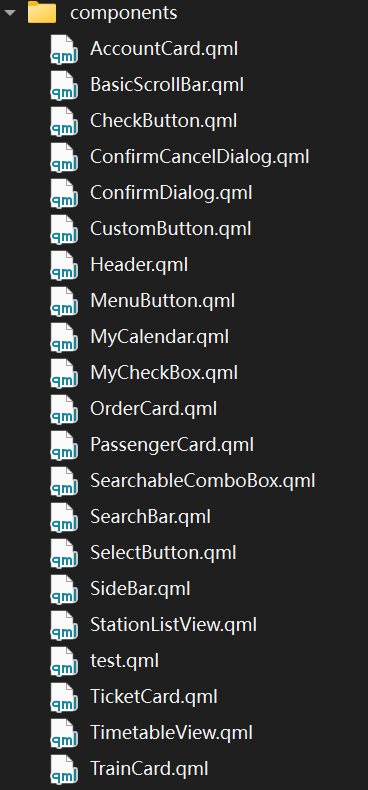
\includegraphics[width=0.4\textwidth]{前端组件.png}
		\caption{前端组件}
		\label{前端组件}
	\end{figure}
	
	所有组件文件全部位于components/目录下，这种组织方式体现了前端开发的模块化设计理念，在开发时考虑到了界面中存在大量可复用的UI元素，比如订单卡片用于展示用户的购票记录、乘车人卡片用于显示乘客信息、自定义按钮如CustomButton和MenuButton用于各种交互操作、滚动条BasicScrollBar和搜索栏SearchBar等组件，这些元素在多个页面中反复出现，如果每次都重新编写代码不仅会增加开发工作量，还容易导致样式不一致和维护困难，因此将它们统一编写成独立的组件文件，并集中放置在components/目录中，不仅便于管理和查找，还通过封装属性和信号实现了高度的代码复用，例如OrderCard组件可以灵活绑定订单数据并处理点击事件，PassengerCard则支持编辑和删除操作，这种设计大大提升了前端代码的可读性和可维护性，同时也确保了整个应用的UI风格统一。
	
	\subsubsection{页面（Pages）}
	\begin{figure}[H]
		\centering
		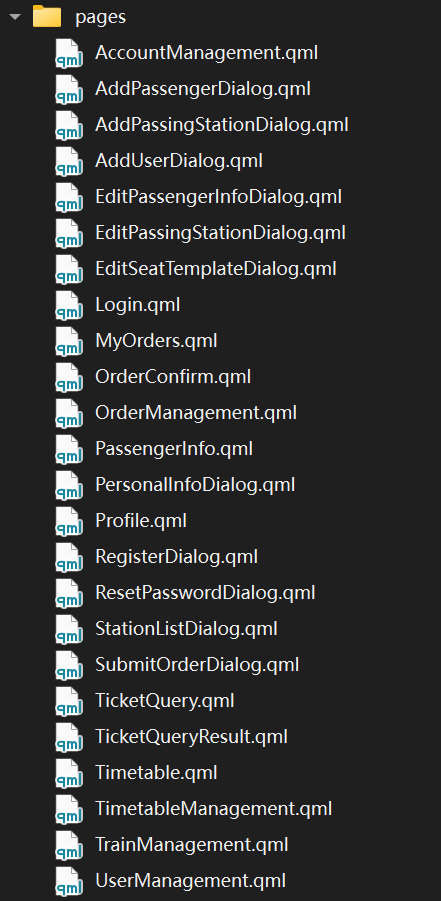
\includegraphics[width=0.4\textwidth]{前端页面.png}
		\caption{前端页面}
		\label{前端页面}
	\end{figure}
	
	所有页面文件全部位于pages/目录下，这种目录结构遵循了前端开发的页面分离原则，高铁管理系统所需的各种界面基本上都以一个独立的文件对应一个页面，例如Login.qml负责用户登录界面、MyOrders.qml展示用户的订单列表、PassengerInfo.qml管理乘车人信息、Profile.qml处理个人资料设置，而像AddPassengerDialog.qml这样的对话框页面则用于添加新乘客的弹窗操作，每个页面文件都通过QML强大的声明式语法进行构建，利用QML对象作为类似HTML标签的基本元素来定义界面组件，如Rectangle、Text、Button等，通过Layout系统如ColumnLayout或RowLayout进行灵活的排版和响应式布局，确保在不同屏幕尺寸下都能良好显示，同时借助QML自带的信号机制、属性绑定和回调函数，以及嵌入的JavaScript逻辑，实现页面间复杂的跳转、弹窗显示和状态切换，例如在MyOrders.qml中点击订单卡片可以触发信号加载Timetable.qml时刻表页面，或者在Profile.qml中确认注销后通过JavaScript清空SessionState并跳转回登录界面。
	
	\subsubsection{前后端通信机制}
	系统在启动阶段，将核心业务对象（如 BookingSystem 以及各类 Manager）通过 QQmlContext 注入到 QML 上下文中，使 QML 可以直接访问这些对象并调用其对外接口。该方式能够避免在 QML 中频繁创建业务对象，也减少了对象传递与生命周期管理的复杂度，保证页面之间调用入口一致，便于统一管理与调试。
	
	对于“从界面发起的动作”（例如查询、下单、取消订单等），使用 Q\_INVOKABLE 将 C++ 方法暴露给 QML，使 QML 能以直观的函数调用方式触发业务逻辑；对于“需要在界面展示且可能变化的数据”（例如当前用户信息、查询结果列表、订单状态等），使用 Q\_PROPERTY 暴露为属性并结合 notify 信号，在数据变化时自动通知界面刷新，从而减少手工更新 UI 的代码量，提升交互的一致性与响应性。
	
	在 C++ 与 QML 的数据交互中，采用 QVariantMap（键值结构）与 QVariantList（列表结构）作为通用数据容器，能够以较低成本承载多字段、可变结构的数据（如车次条目、订单条目、乘车人信息等），并与 QML/JS 的对象与数组结构天然匹配，便于在界面侧直接遍历、绑定与渲染。相比为每一种展示数据都定义专门的类与模型，这种方式更轻量、字段扩展更灵活，适合需求迭代阶段快速调整显示字段与接口返回结构，同时也能统一不同模块的数据返回形式，降低前后端对接成本。
	
	\subsection{类图}
	\begin{figure}[H]
		\centering
		\includesvg[width=0.9\textheight, angle=270]{类图.svg}
		\caption{类图}
		\label{类图}
	\end{figure}
	
	\subsection{关键顺序图}
	\begin{figure}[H]
		\centering
		\includesvg[width=0.7\textwidth]{顺序图-登录.svg}
		\caption{顺序图-登录}
		\label{顺序图-登录}
	\end{figure}
	\begin{figure}[H]
		\centering
		\includesvg[width=0.7\textwidth]{顺序图-注册.svg}
		\caption{顺序图-注册}
		\label{顺序图-注册}
	\end{figure}
	\begin{figure}[H]
		\centering
		\includesvg[width=0.6\textwidth]{顺序图-查询历史.svg}
		\caption{顺序图-查询历史}
		\label{顺序图-查询历史}
	\end{figure}
	\begin{figure}[H]
		\centering
		\includesvg[width=0.7\textwidth]{顺序图-查询余票.svg}
		\caption{顺序图-查询余票}
		\label{顺序图-查询余票}
	\end{figure}
	\begin{figure}[H]
		\centering
		\includesvg[width=0.7\textwidth]{顺序图-预订车票.svg}
		\caption{顺序图-预订车票}
		\label{顺序图-预订车票}
	\end{figure}
	\begin{figure}[H]
		\centering
		\includesvg[width=0.7\textwidth]{顺序图-我的订单.svg}
		\caption{顺序图-我的订单}
		\label{顺序图-我的订单}
	\end{figure}
	\begin{figure}[H]
		\centering
		\includesvg[width=0.7\textwidth]{顺序图-查看订单时刻表.svg}
		\caption{顺序图-查看订单时刻表}
		\label{顺序图-查看订单时刻表}
	\end{figure}
	\begin{figure}[H]
		\centering
		\includesvg[width=0.7\textwidth]{顺序图-乘车人信息.svg}
		\caption{顺序图-乘车人信息}
		\label{顺序图-乘车人信息}
	\end{figure}
	\begin{figure}[H]
		\centering
		\includesvg[width=0.7\textwidth]{顺序图-取消订单.svg}
		\caption{顺序图-取消订单}
		\label{顺序图-取消订单}
	\end{figure}
	\begin{figure}[H]
		\centering
		\includesvg[width=0.7\textwidth]{顺序图-修改乘车人信息.svg}
		\caption{顺序图-修改乘车人信息}
		\label{顺序图-修改乘车人信息}
	\end{figure}
	\begin{figure}[H]
		\centering
		\includesvg[width=0.7\textwidth]{顺序图-删除乘车人信息.svg}
		\caption{顺序图-删除乘车人信息}
		\label{顺序图-删除乘车人信息}
	\end{figure}
	\begin{figure}[H]
		\centering
		\includesvg[width=0.7\textwidth]{顺序图-添加乘车人信息.svg}
		\caption{顺序图-添加乘车人信息}
		\label{顺序图-添加乘车人信息}
	\end{figure}
	\begin{figure}[H]
		\centering
		\includesvg[width=0.7\textwidth]{顺序图-修改个人信息.svg}
		\caption{顺序图-修改个人信息}
		\label{顺序图-修改个人信息询历史}
	\end{figure}
	\begin{figure}[H]
		\centering
		\includesvg[width=0.7\textwidth]{顺序图-用户注销.svg}
		\caption{顺序图-用户注销}
		\label{顺序图-用户注销}
	\end{figure}
	\begin{figure}[H]
		\centering
		\includesvg[width=0.7\textwidth]{顺序图-车次管理.svg}
		\caption{顺序图-退出登录}
		\label{顺序图-退出登录}
	\end{figure}
	\begin{figure}[H]
		\centering
		\includesvg[width=0.7\textwidth]{顺序图-车次管理时刻表.svg}
		\caption{顺序图-车次管理时刻表}
		\label{顺序图-车次管理时刻表}
	\end{figure}
	\begin{figure}[H]
		\centering
		\includesvg[width=0.7\textwidth]{顺序图-删除列车.svg}
		\caption{顺序图-删除列车}
		\label{顺序图-删除列车}
	\end{figure}
	\begin{figure}[H]
		\centering
		\includesvg[width=0.7\textwidth]{顺序图-添加列车.svg}
		\caption{顺序图-添加列车}
		\label{顺序图-添加列车}
	\end{figure}
	\begin{figure}[H]
		\centering
		\includesvg[width=0.7\textwidth]{顺序图-订单管理.svg}
		\caption{顺序图-订单管理}
		\label{顺序图-订单管理}
	\end{figure}
	\begin{figure}[H]
		\centering
		\includesvg[width=0.7\textwidth]{顺序图-改签.svg}
		\caption{顺序图-改签}
		\label{顺序图-改签}
	\end{figure}
	\begin{figure}[H]
		\centering
		\includesvg[width=0.7\textwidth]{顺序图-退票.svg}
		\caption{顺序图-退票}
		\label{顺序图-退票}
	\end{figure}
	\begin{figure}[H]
		\centering
		\includesvg[width=0.7\textwidth]{顺序图-用户管理.svg}
		\caption{顺序图-用户管理}
		\label{顺序图-用户管理}
	\end{figure}
	\begin{figure}[H]
		\centering
		\includesvg[width=0.7\textwidth]{顺序图-重置密码.svg}
		\caption{顺序图-重置密码}
		\label{顺序图-重置密码}
	\end{figure}
	\begin{figure}[H]
		\centering
		\includesvg[width=0.7\textwidth]{顺序图-锁定.svg}
		\caption{顺序图-锁定}
		\label{顺序图-锁定}
	\end{figure}
	\begin{figure}[H]
		\centering
		\includesvg[width=0.7\textwidth]{顺序图-解锁.svg}
		\caption{顺序图-解锁}
		\label{顺序图-解锁}
	\end{figure}
	
	
	\subsection{关键活动图}
	\begin{figure}[H]
		\centering
		\includesvg[width=0.7\textwidth]{活动图-预订车票.svg}
		\caption{活动图-预订车票}
		\label{活动图-预订车票}
	\end{figure}
	\begin{figure}[H]
		\centering
		\includesvg[width=0.7\textwidth]{活动图-修改乘车人信息.svg}
		\caption{活动图-修改乘车人信息}
		\label{活动图-修改乘车人信息}
	\end{figure}
	\begin{figure}[H]
		\centering
		\includesvg[width=0.7\textwidth]{活动图-系统.svg}
		\caption{活动图-系统}
		\label{活动图-系统}
	\end{figure}
	
	\section{主要功能算法设计}
	\subsection{余票查询功能设计}
	该功能的目标是：在用户给定出发城市、到达城市与出行日期的情况下，返回所有满足“从出发城市到达目的城市”的车次方案，并计算每个方案在该日期下的各席别余票数量、发到时间、历时与票价，最终以列表形式返回给 QML 侧展示。
	
	整体流程如下：
	
	\paragraph{依赖检查} 首先检查 StationManager / TrainManager / OrderManager / AccountManager 等核心管理模块是否已正确初始化。若存在空指针，直接返回空列表，避免后续计算出错。
	
	\paragraph{获取可达车次方案（候选路线集合）} 调用 TrainManager::getRoutesByCities(startCityName, endCityName) 获取所有候选方案。
	每个方案包含三部分：
	\begin{itemize}
		\item Train：车次对象（含车次号、座位配置、时刻表等）
		\item startStation：该车次在出发城市对应的上车站点
		\item endStation：该车次在到达城市对应的下车站点
	\end{itemize}
	这样能确保后续计算是针对“同一车次内的一个出发站—到达站区间”。
	
	\paragraph{读取该车次各席别总座位数作为初始余票} 从 Train 中取出一等座、二等座、商务座的座位总数，分别作为 first/second/business 的初始余票计数。
	
	\paragraph{计算该区间的出发/到达日期时间范围} 从车次 Timetable 中分别取出出发站与到达站的时刻信息（到/发时刻、跨天信息、停靠信息等）。出发时间取出发站的“发车时刻”，到达时间取到达站的“到达时刻”。根据时刻表记录的跨天偏移（代码中通过 endStationInfo 与 startStationInfo 的天数偏移差计算），得到本次查询对应的 queryEndDate。这样就得到该区间对应的完整时间窗口：trainNumber + [queryStartDate queryStartTime, queryEndDate queryEndTime]。
	
	\paragraph{查找与该区间时间窗口重叠且未使用的订单} 调用 OrderManager::getOrdersUnusedAndOverlapByTrainNumber(...)，按以下条件筛选订单：
	\begin{itemize}
		\item 同一车次号
		\item 订单状态为“未使用/有效”（未乘车且未作废）
		\item 订单乘车时间区间与本次查询区间存在重叠（Overlap）
	\end{itemize}
	这些订单会占用本次区间的座位资源，需要从余票中扣减。
	
	\paragraph{按席别扣减余票} 遍历所有重叠订单：
	\begin{itemize}
		\item 若订单席别为“一等座”，则 firstClassCount--
		\item 若为“二等座”，则 secondClassCount--
		\item 若为“商务座”，则 businessClassCount--
	\end{itemize}
	遍历完成后，得到该日期该区间的实际余票数。
	
	\paragraph{组织返回结果} 将车次号、出发/到达站名、出发/到达日期时间、历时（由时刻表计算区间秒数再转小时分钟）、票价（调用 computePrice）、以及三种席别余票数量一起封装成 QVariantMap，加入返回列表。
	\newline
	
	\begin{lstlisting}[language=C++, caption={查询余票算法伪代码}]
		// 关键目标：计算指定日期(startDate)下，所有可行车次方案的各席别余票
		// 余票 = 该车次席别总座位数 - 与该区间“时间重叠且未使用”的订单数（按席别分别扣减）
		
		struct TicketResult {
			string trainNo;
			int firstRemain;
			int secondRemain;
			int businessRemain;
			// 关键展示字段可保留：出发/到达时间、历时等（此处省略）
		};
		
		vector<TicketResult> queryTickets(string startCity, string endCity, Date startDate)
		{
			vector<TicketResult> results;
			
			// 1) 获取所有可达方案：每个方案给出(train, startStation, endStation)
			vector<Route> routes = TrainManager_getRoutesByCities(startCity, endCity);
			
			for (Route r : routes) {
				
				Train train = r.train;
				Station A = r.startStation;
				Station B = r.endStation;
				Timetable tt = train.timetable;
				
				// 2) 初始化余票 = 座位总数
				int firstRemain    = train.firstClassCount;
				int secondRemain   = train.secondClassCount;
				int businessRemain = train.businessClassCount;
				
				// 3) 计算该区间的出发/到达日期时间窗口（用于判定订单是否占座）
				StationInfo aInfo = tt.getStationInfo(A.name);
				StationInfo bInfo = tt.getStationInfo(B.name);
				
				Time departTime = aInfo.departTime;     // 出发站“发车时刻”
				Time arriveTime = bInfo.arriveTime;     // 到达站“到达时刻”
				int dayOffset = bInfo.dayOffset - aInfo.dayOffset;  // 跨天差
				Date endDate = startDate + dayOffset;
				
				// 4) 找出同车次、未使用、且与该区间时间窗口重叠的订单
				vector<Order> overlapOrders =
				OrderManager_getUnusedOverlapOrders(train.number,
				startDate, departTime,
				endDate, arriveTime);
				
				// 5) 按订单席别扣减余票
				for (Order o : overlapOrders) {
					if (o.seatLevel == FIRST_CLASS)      firstRemain--;
					else if (o.seatLevel == SECOND_CLASS) secondRemain--;
					else if (o.seatLevel == BUSINESS)     businessRemain--;
				}
				
				// 6) 输出关键结果（只保留关键字段）
				TicketResult item;
				item.trainNo = train.number;
				item.firstRemain = firstRemain;
				item.secondRemain = secondRemain;
				item.businessRemain = businessRemain;
				
				results.push_back(item);
			}
			
			return results;
	}			\end{lstlisting}
	
	\subsection{提交订单功能设计}
	用户在车票查询界面点击某个车票的预订按钮后，首先需要查询该用户下所有空闲乘车人，由用户选择哪些乘车人后，再对每个乘车人生成一个订单。算法描述如下：
	
	\paragraph{查询空闲乘车人} 入口函数为 \texttt{BookingSystem::getPassengers\_api}（前端传入 \texttt{username} 以及本次行程的起止日期/时间窗口）。后端首先根据 \texttt{username} 获取该用户下的全部乘车人列表；随后对每个乘车人 \texttt{passenger} 调用 \texttt{OrderManager::isPassengerAvailable(passengerId, window)} 判断其在该窗口内是否空闲。可用性判断仅考虑该乘车人名下 \texttt{status} 为 \texttt{"待乘坐"} 的订单（\texttt{"已取消"}、\texttt{"已改签"}、\texttt{"已乘坐"} 不参与占用计算）；若存在任意一张 \texttt{"待乘坐"} 订单与本次查询窗口发生时间区间重叠，则该乘车人判定为不可用。最终返回前端一个列表，每项包含乘车人基本信息及 \texttt{available} 布尔值，用于界面端的置灰或提示。时间冲突判定的底层逻辑由 \texttt{Order::isTimeRangeOverlap} 实现：
	\begin{itemize}
		\item 先按日期判断两区间是否完全不相交：若 \texttt{orderEndDate < queryStartDate} 或 \texttt{queryEndDate < orderStartDate}，则不重叠；
		\item 若日期存在交集，再处理同日边界情况：
		\begin{itemize}
			\item 若 \texttt{orderEndDate == queryStartDate} 且 \texttt{orderEndTime < queryStartTime}，则不重叠（订单在查询前结束）；
			\item 若 \texttt{queryEndDate == orderStartDate} 且 \texttt{queryEndTime < orderStartTime}，则不重叠（查询在订单前结束）；
		\end{itemize}
		\item 其余情况均视为重叠。
	\end{itemize}
	
	\paragraph{提交订单} 提交订单由 \texttt{BookingSystem::createOrder\_api} 统一完成，前端传入用户名、车次号、乘车人、起终站、日期、席别及可选的待改签订单号。函数首先对关键参数与实体进行校验（用户、车次、乘车人、站点等），并区分普通购票与改签两种模式：普通购票以传入用户名作为订单归属，改签则以原订单中的用户名为准以避免归属不一致。随后根据列车时刻表计算本次行程的精确出发/到达日期时间窗口，并调用订单模块扫描同车次、同席别、状态为“待乘坐”且与该窗口重叠的订单，生成不可用座位集合（改签时需排除原订单自身占座）。在此基础上构建座位三维可用表，按车厢号、行、列的顺序采用首次适配策略选择第一个可用座位。票价方面先计算区间基础票价，再依据乘客类型应用折扣得到最终价格。最后创建新订单并生成新的订单号写入订单集合；若为改签场景，则将原订单状态更新为“已改签”。
	\newline
	
	\begin{lstlisting}[language=C++, caption={提交订单伪代码}]
		// 1) 查询空闲乘车人：给前端返回 available 标记
		QVariantList GetPassengers_api(username, window) {
			list = {}
			for (Passenger p : passengerMgr.getByUsername(username)) {
				bool ok = orderMgr.isPassengerAvailable(p.id, window)   // 只看“待乘坐”且时间重叠则不可用
				list.push({ name:p.name, id:p.id, type:p.type, available:ok })
			}
			return list
		}
		
		// 2) 提交订单：校验 -> 算窗口 -> 占座 -> 选座 -> 计价 -> 落单（可改签）
		QVariantMap CreateOrder_api(info) {
			// 校验实体存在（用户/车次/乘车人/车站，改签订单可选）
			User user = ResolveUser(info.username, info.pendingRescheduleOrderNumber)
			Train train = trainMgr.getTrain(info.trainNumber)
			Passenger p = passengerMgr.getByUsernameAndId(user.username, info.passengerId)
			Station s = stationMgr.getStation(info.startStationName)
			Station e = stationMgr.getStation(info.endStationName)
			
			// 用时刻表计算精确时间窗口（含跨天）
			Window w = BuildWindow(info.date, train.timetable, s, e)
			
			// 统计同车次同席别、且与 w 重叠的“待乘坐”订单座位 -> 标记占用
			occ = orderMgr.getUnavailableSeats(train.no, info.seatLevel, w, info.pendingRescheduleOrderNumber)
			seats = Build3DBool(train.carriages, true);  MarkFalse(seats, occ)
			
			// 首次适配选座（车厢/行/列从小到大找第一个 true）
			SeatPos pos = FirstFit(seats, train.carriages, info.seatLevel)
			if (!pos.found) return Fail("无可用座位")
			
			// 计价：基础票价(席别) * 折扣(成人/儿童/学生)
			price = BasePrice(train.no, s, e, info.seatLevel) * Discount(p.type)
			
			// 创建订单并入库；改签则把原订单标记“已改签”
			Order o = NewOrder(train.no, p, price, w, s, e, info.seatLevel, pos, "待乘坐", user.username)
			orderMgr.createOrder(o)
			if (info.pendingRescheduleOrderNumber != "") orderMgr.reschedule(info.pendingRescheduleOrderNumber)
			return Ok("预定成功")
	}			\end{lstlisting}
	
	\subsection{用户注销功能设计}
	实现“用户注销”（账号删除）时的数据一致性清理：在删除账号前，先删除其关联的订单与乘车人信息，避免系统残留无主数据；最终向前端返回 \texttt{success/message}。输入为前端传入的 \texttt{QVariantMap info}，其中包含 \texttt{username}。输出为 \texttt{QVariantMap result}，至少包含 \texttt{success}（布尔值）与 \texttt{message}（字符串）。核心流程如下：
	
	\paragraph{检查用户是否存在} 注销入口从 \texttt{info} 中读取用户名，即 \texttt{username = info["username"].toString()}。随后调用 \texttt{account\_manager->getUserByUsername(username)} 检查账户是否存在：若返回 \texttt{std::nullopt}，则直接构造失败结果并返回（\texttt{success=false}，\texttt{message="用户不存在"}）；若用户存在，则进入清理阶段。
	
	\paragraph{用户数据清理} 清理阶段依次执行三步。第一步调用 \texttt{order\_manager->deleteOrdersByUsername(username)} 删除该用户的全部订单。其实现为遍历内存中的 \texttt{orders} 容器，通过迭代器逐项比较 \texttt{order.getUsername()} 与目标 \texttt{username}；匹配则执行 \texttt{erase(it)} 删除并继续迭代，不匹配则迭代器后移。第二步调用 \texttt{passenger\_manager->deletePassengersByUsername(username)} 删除该用户的全部乘车人信息，算法结构与订单删除相同：遍历 \texttt{passengers}，比较 \texttt{passenger.getUsername()}，匹配后 \texttt{erase(it)}。第三步调用 \texttt{account\_manager->deleteUser(username)} 删除用户账号；该函数遍历 \texttt{users} 容器，匹配 \texttt{user.getUsername()} 后执行 \texttt{erase(it)} 并返回 \texttt{true}。
	
	\paragraph{返回结果} 当上述步骤完成后，接口层返回成功结果：\texttt{success=true}，并设置提示信息为 \texttt{message="用户 X 注销成功"}。
	\newline
	
	\begin{lstlisting}[language=C++, caption={用户注销功能伪代码}]
		QVariantMap DeleteUser_api(QVariantMap info) {
			QString u = info["username"].toString();
			if (!accountMgr.getUserByUsername(u)) return {{"success",false},{"message","用户不存在"}};
			
			orderMgr.deleteOrdersByUsername(u);        // 删除所有订单中 order.username == u 的记录
			passengerMgr.deletePassengersByUsername(u);// 删除所有乘车人中 passenger.username == u 的记录 passenger.username==u
			accountMgr.deleteUser(u);                  // 删除用户表中 user.username == u 的记录
			
			return {{"success",true},{"message", QString("用户 %1 注销成功！").arg(u)}};
	}			\end{lstlisting}
	
	\section{前端开发}
	\subsection{总体设计}
	本项目前端用 QML 编写，程序从 \texttt{main.qml} 启动。为了让“当前是谁在用、有没有登录、属于用户还是管理员”这些信息在各页面之间共享，我们把它们统一放在 \texttt{SessionState.qml} 里管理。页面需要数据时，就直接调用后端提供的接口（例如 \texttt{bookingSystem}、\texttt{accountManager}、\texttt{orderManager}、\texttt{stationManager}），拿到结果后刷新界面即可。
	
	页面安排基本按用户的实际操作顺序来走：先查票，再下单，然后去订单里查看或处理；管理员则负责维护车次、订单和账号。这样做的目的很简单：让使用过程更顺，不用来回跳很多页面。至于“能看什么、能做什么”，主要由 \texttt{SessionState} 决定：一旦角色确定，页面入口和菜单就跟着切换，从而避免在同一个页面里写太多“如果是管理员就显示这个，否则显示那个”的判断。
	
	主窗口会根据 \texttt{SessionState.role} 选择默认页面：管理员直接进入 \texttt{TrainManagement.qml}，普通用户进入 \texttt{TicketQuery.qml}。左侧菜单由 \texttt{SideBar.qml} 根据角色生成：管理员看到“车次/订单/账户”，用户看到“查询/乘车人/我的订单”。角色分流主要在这里完成，其它页面只专心做自己的事情。
	
	\begin{figure}[H]
		\centering
		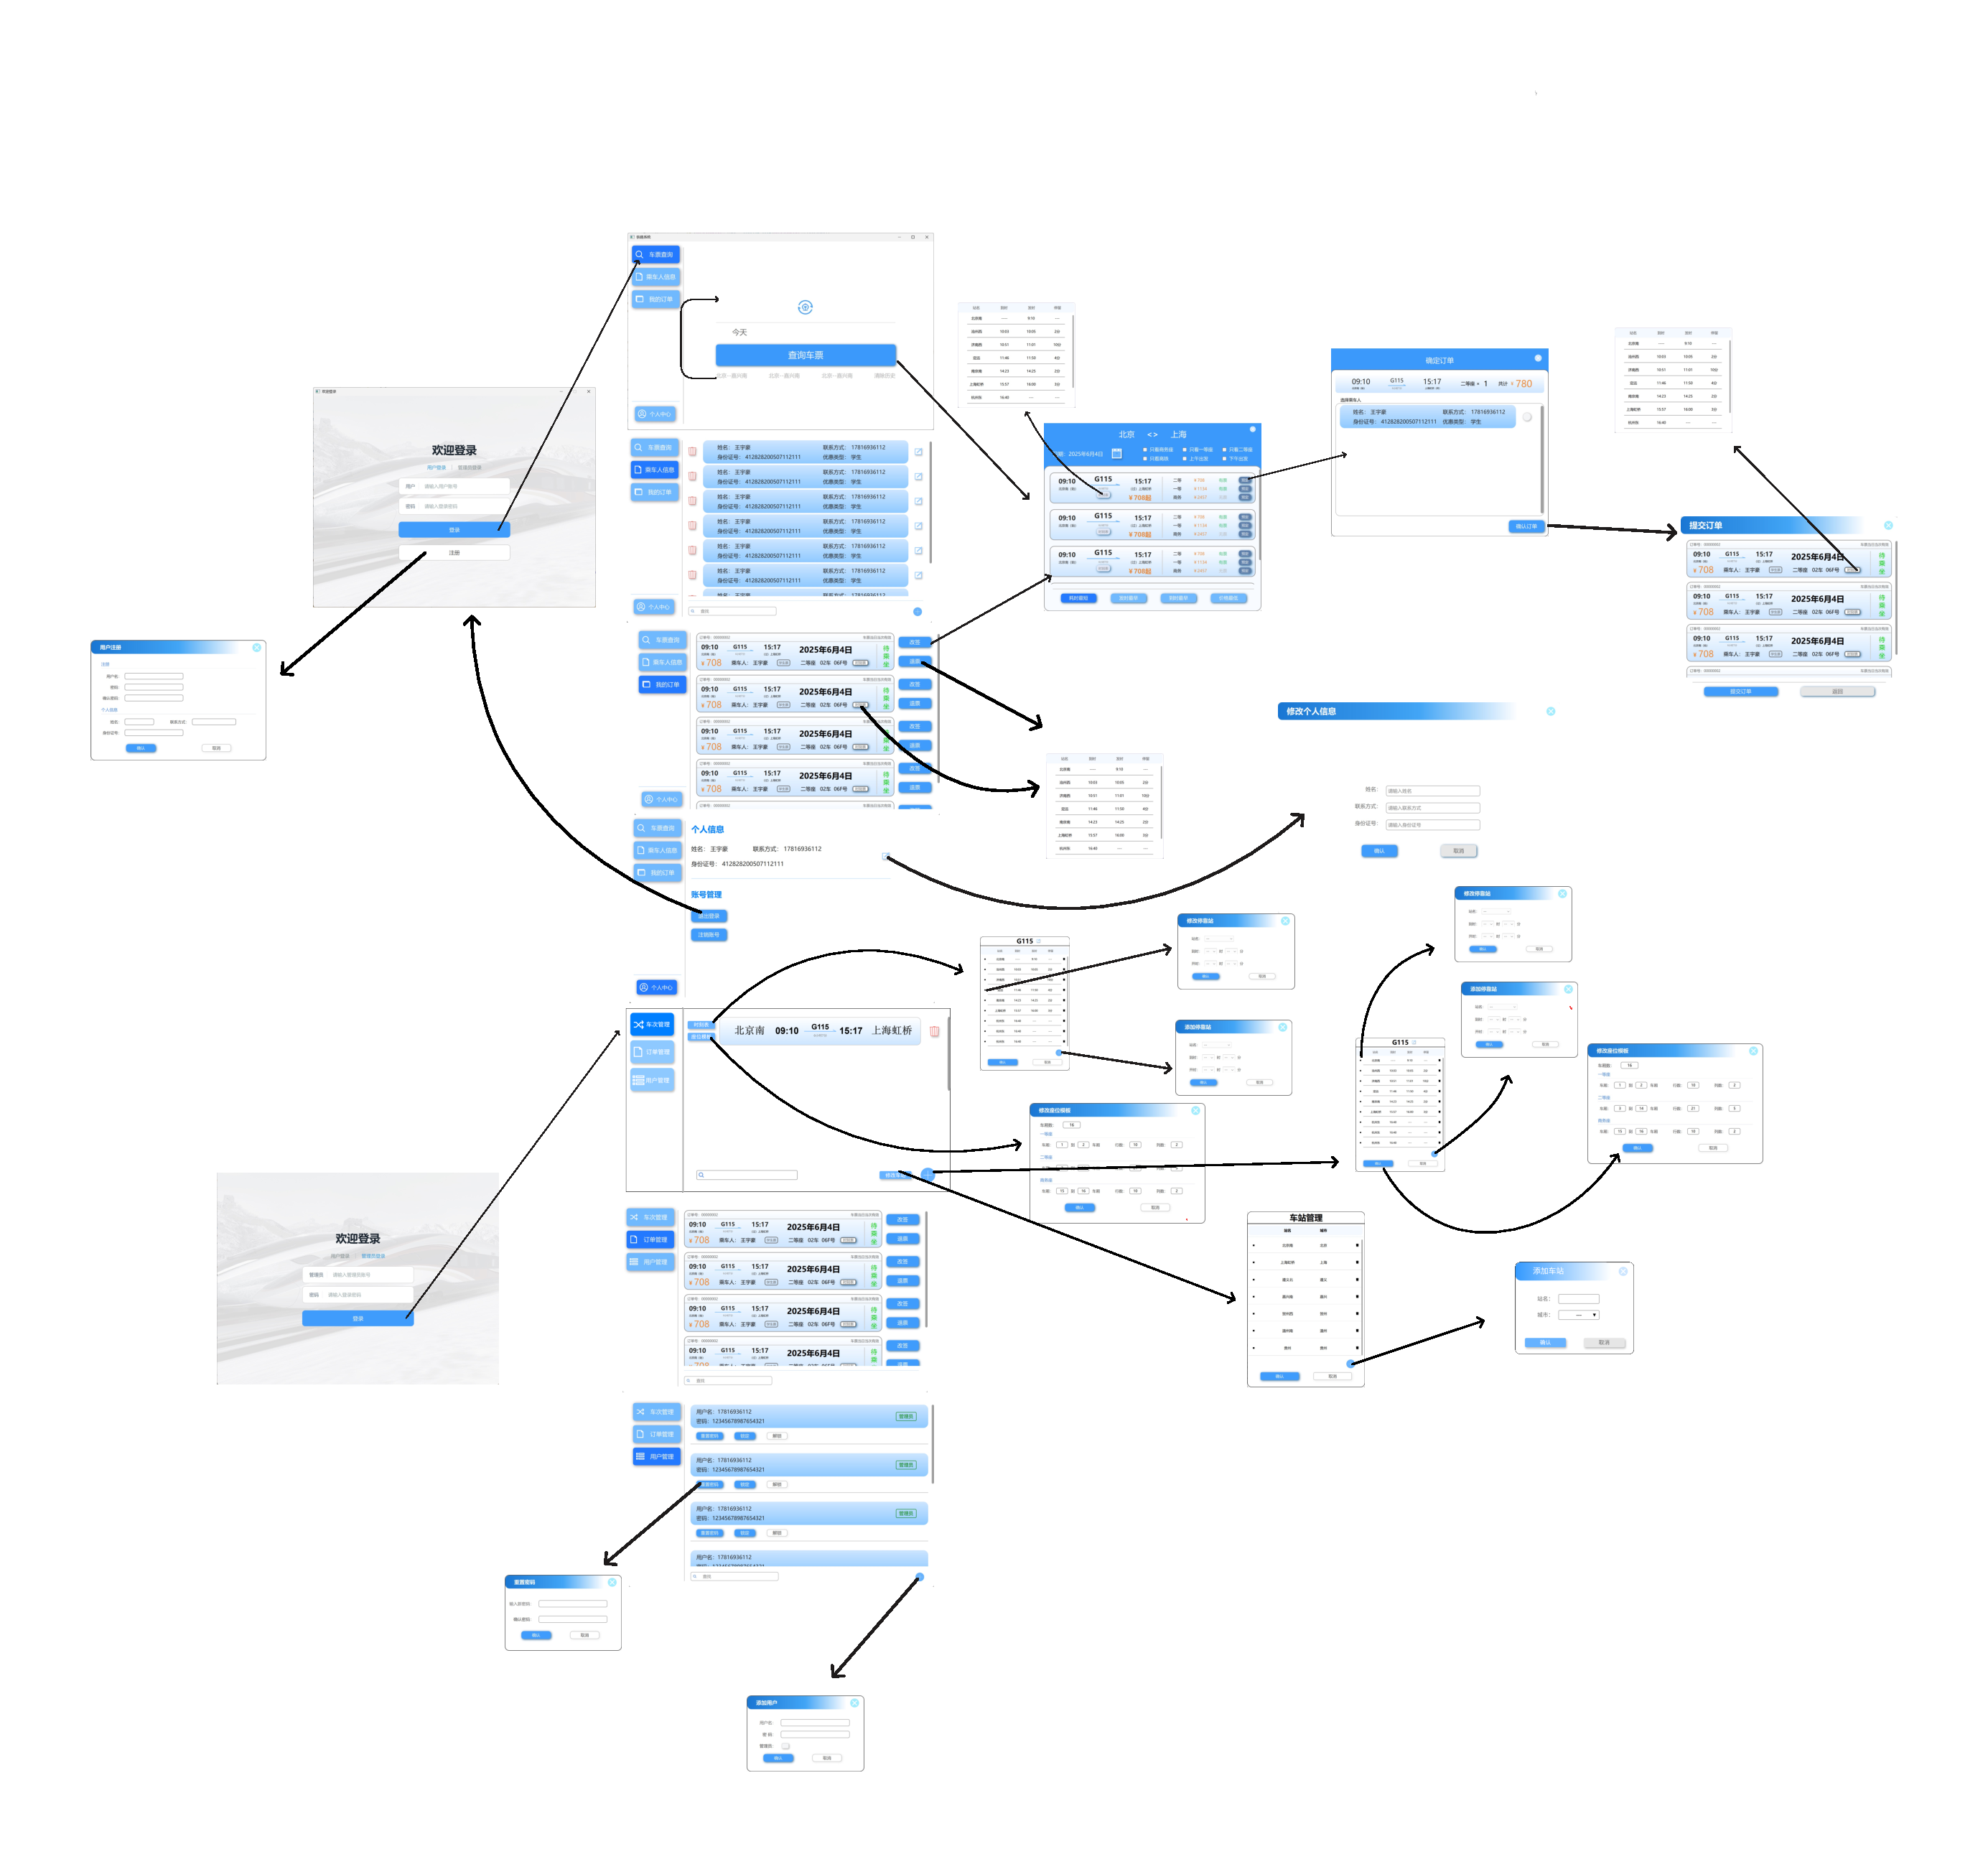
\includegraphics[width=\textwidth]{页面跳转逻辑图.pdf}
		\caption{页面跳转逻辑图}
	\end{figure}
	
	\subsection{登录界面}
	登录页 \texttt{Login.qml} 是一个可嵌入的页面，由 \texttt{main.qml} 用 \texttt{Loader} 覆盖在主界面之上。用户可以在“用户登录/管理员登录”之间切换（\texttt{isAdminLogin}），界面会用颜色和字体变化提示当前模式。点击登录后分别调用 \texttt{accountManager.loginUser\_api(...)} 或 \texttt{accountManager.loginAdmin\_api(...)}。登录成功就把 \texttt{SessionState.role} 和 \texttt{SessionState.username} 写进去，再把 \texttt{SessionState.isLoggedIn} 置为 \texttt{true}，随后触发 \texttt{loadStartPage()} 跳到对应的起始页（加一点延时是为了让页面容器先准备好）。
	
	\subsection{订单流程页面（从查询到提交）}
	整个订票流程从 \texttt{TicketQuery.qml} 开始。页面会先从 \texttt{stationManager.getCitiesName\_api()} 拿到城市列表，用户选择出发地和目的地后点击查询；同时会调用 \texttt{bookingSystem.addQueryHistory\_api(from,to)} 记一条查询历史，方便下次复用。查询结果在 \texttt{TicketQueryResult.qml} 里展示，它用一个独立的 \texttt{Window} 弹出来并设为模态（\texttt{Qt.WindowModal}），这样用户不会在中途跑去点其它页面导致流程断掉。筛选与排序主要在前端对结果列表做处理，减少重复请求；如果是改签模式（\texttt{rescheduleMode=true}），一些容易误操作的交互（比如交换出发/到达）会被禁用，并给出相应的鼠标提示。
	
	选中车次后进入确认窗口 \texttt{OrderConfirm.qml}：这里把“车票信息、乘车人选择、价格展示”集中在一处完成。普通购票会调用 \texttt{bookingSystem.getPassengers\_api(\{...\})}，后端会给出每个乘车人在该时间段是否可用的标记 \texttt{available}；改签场景则调用 \texttt{orderManager.getPassengerForReschedule\_api(...)}，直接加载原订单对应的乘车人并尽量默认选中。界面上不可用的乘车人会提示原因，相关按钮也会自动变灰并禁止点击；总价会随勾选即时更新，给用户一个直观反馈。
	
	最后是提交弹窗 \texttt{SubmitOrderDialog.qml}，采用无边框样式并支持拖动，桌面端体验更自然。点击“提交订单”会调用 \texttt{bookingSystem.createOrder\_api(\{...\})} 完成落单；改签时管理员端不会强行传 \texttt{username}，由后端从待改签订单反查归属，减少传参不一致带来的问题。提交结束会弹出提示，并通过信号通知上层刷新列表或关闭窗口。
	
	\subsection{订单管理界面（用户/管理员）}
	用户端的“我的订单”在 \texttt{MyOrders.qml} 中实现，用 \texttt{ListView} 配合 \texttt{OrderCard} 以卡片形式展示，滚动条样式统一。订单卡片提供改签与退票等操作，并按状态做限制：只有 \texttt{status=="待乘坐"} 的订单才允许改签；退票会先弹出确认框，避免误点。页面还提供多条件搜索（订单号、车次、日期、乘车人、站点），订单多的时候更好找。
	
	管理员端 \texttt{OrderManagement.qml} 的界面结构与用户端基本一致，复用同一套卡片与搜索方式，主要区别在于数据是全量订单；操作同样有状态限制和确认弹窗，保证处理逻辑一致。
	
	\subsection{管理员后台页面}
	车次管理页 \texttt{TrainManagement.qml} 用 \texttt{TrainCard} 展示车次列表，并提供时刻表、座位模板与删除等入口。删除前会先做可编辑性检查（例如 \texttt{isTrainEditable(...)}），如果车次存在风险（如仍有关联的待乘坐订单）则直接阻止删除并提示原因。编辑相关功能采用 \texttt{Loader} 按需加载弹窗（时刻表管理、座位模板编辑等），主页面保持简洁，也能减少卡顿。
	
	账户管理页 \texttt{UserManagement.qml} 用 \texttt{AccountCard} 展示账号信息，提供重置密码、锁定、解锁等操作。危险操作统一要二次确认，并且做了基本的防呆：例如管理员不能锁定自己（当 \texttt{SessionState.username == modelData.username} 时直接拦截并提示）。
	
	\subsection{页面组织与导航（StackView + Loader）}
	主内容区由 \texttt{StackView} 承载。侧边栏点击菜单后会清空当前栈并进入目标页面（\texttt{stackView.clear(); stackView.push(pageUrl, \{...\})}），同时在 \texttt{onCurrentItemChanged} 中同步菜单选中态，保证“当前页”和“菜单高亮”一致。登录页则用 \texttt{Loader} 覆盖主界面：未登录时把主内容遮住，登录成功后再移除覆盖层，避免出现页面还没准备好就被误操作的情况。
	
	\section{总结与感想}
	我们二人团队从暑假开始起草需求、绘制前端原型与页面结构，十月份集中完成前端开发，十一月份再推进后端实现与联调，完整经历了一个小型软件项目从设计到落地的全过程。期间我们学习并实际使用了两门新技术：\texttt{QML} 与 \texttt{JavaScript}。其中，\texttt{QML} 作为一种偏界面描述的语言，写起来接近“搭积木”，能快速做出结构清晰、交互自然的桌面界面；而它对 \texttt{JavaScript} 的支持也让我们能在界面侧完成筛选、排序、即时反馈等逻辑，显著提升了开发效率与可用性体验。同时，在版本控制的约束下，我们也更熟练地使用了 \texttt{Git}：学会用分支隔离开发、用提交记录定位问题、用合并解决冲突，并把协作流程逐步做得更规范。
	
	也许一年两年之后，我们会淡忘项目的具体架构、某个页面的布局细节，甚至记不清 \texttt{QML} 的语法习惯；但我们不会忘记那些为了对齐接口、排查 bug、反复测试而忙到深夜的日子。它们让我们更清楚地认识到：软件开发从来不是把代码写出来那么简单，而是一段不断试错、不断靠近正确答案的过程。
	
	未来无论我们走向哪种方向，这段完整的项目经历都会提醒我们保持耐心、保持沟通、保持对质量的敬畏，并把每一次困难都当作下一次更成熟开发的起点……
\end{document}